\documentclass{article}
%\usepackage{fullpage}
%\usepackage{fullpage}
\usepackage{amsmath}
\usepackage{tikz}
\usepackage{latexsym}
\usepackage{amssymb,amsfonts}
\usepackage{graphicx}
\usepackage{array}
\usepackage{graphics}
\usepackage{wrapfig}
\usepackage{multirow}
\usepackage[margin=.75in]{geometry}

\newcommand{\fillinblank}{ \line(1,0){100} }

\setlength{\parindent}{0.3in}
\setlength{\parskip}{0.1in}

\pagenumbering{gobble}

\begin{document}
\begin{flushleft}
\begin{tabular}{l c r}
 \begin{tabular}{l}
   {\Huge MaPP-Callenge 2020}\\
   {\Huge Gerrymandering Puzzle }\\
   {\Large (Idea/Draft)}
   \end{tabular}
    \begin{tabular}{c}
   \hspace{1in}
   \end{tabular}
   
\end{tabular}\begin{tabular}{r}
     
\includegraphics[width=2in]{mapp-square.pdf}
 \end{tabular}
   

\thispagestyle{empty}

\noindent\hrulefill
\phantom{.}\vspace{.15in}

Indiana Jones has come across ancient archives of election results of a long forgotten democratic civilization. Blah blah story about how he found this.... The civilization was made up of six provinces who were each given a specific number of representatives at the Kings council. We have three years of election data where party X sent the most representatives to the king's council in each province every year, even though they never received the most number of votes in that province. HOW COULD THIS BE? The elections were conducted by dividing each province into districts and the candidate who obtained the majority vote in a district was sent to represent the district at the king's council. Since the members of the provinces moved there houses so frequently, the district lines were re-drawn each year according to the following guidelines.

\textbf{District drawing rules}
\begin{enumerate}
\item No district's population can exceed any others by more than 5 people.
\item All district lines must follow the grid lines provided
\item All districts must be connected (not necessarily simply connected)
\end{enumerate}


We know that each year the prince of the province was able to re-draw the district lines, however the number of districts in any particular province never changed. We also know that there was never a time when there was a tie in any district. Your objective is to determine the number a districts in each province to discover the hidden message.

(We should make up some scheme such as adding the number of districts to the letter of the province in a cypher. We could also give the name of the Prince in each city, and then take the letter in the position of the name that corresponds with the number of districts needed. Whatever we do to decode the message should be sufficiently hidden, so that they need to fully explore drawing the districts.)

\newpage
Province A \\
Population = 50
\begin{tabular}{c c c }

Year 1 & Year 2 & Year 3 \\
 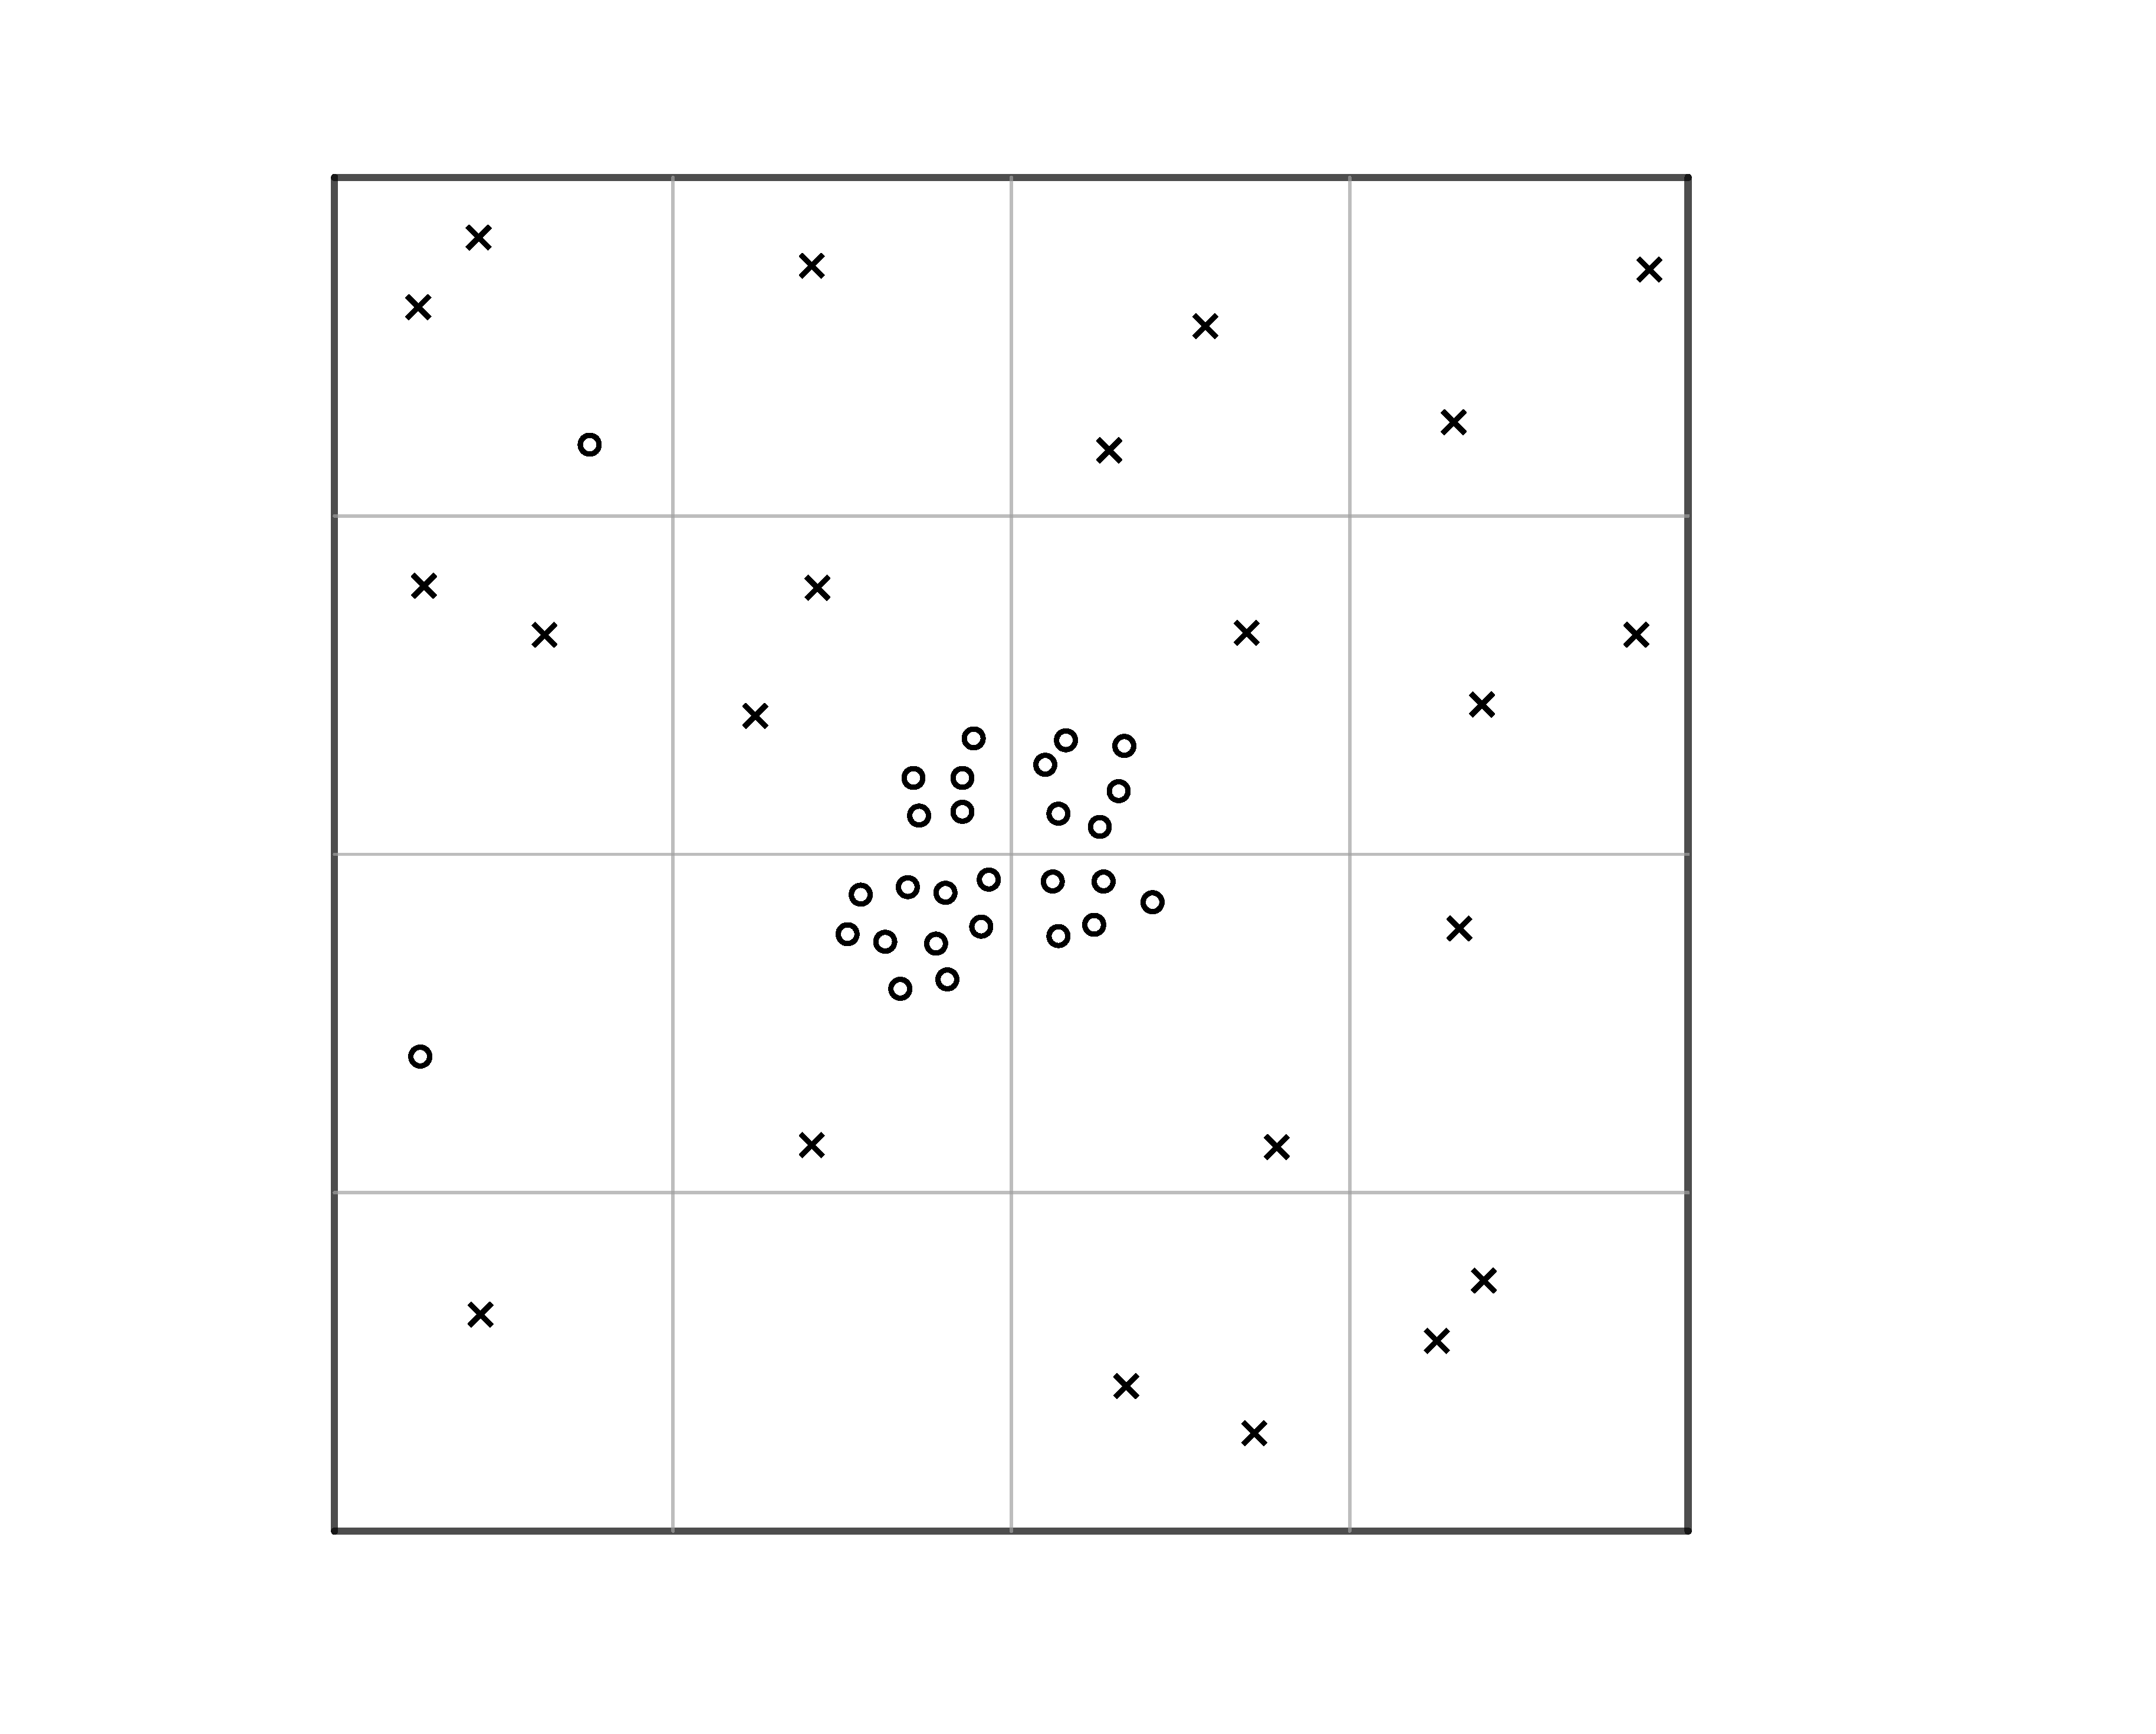
\includegraphics[width=2in]{Gerry4x4-50-1.pdf} &  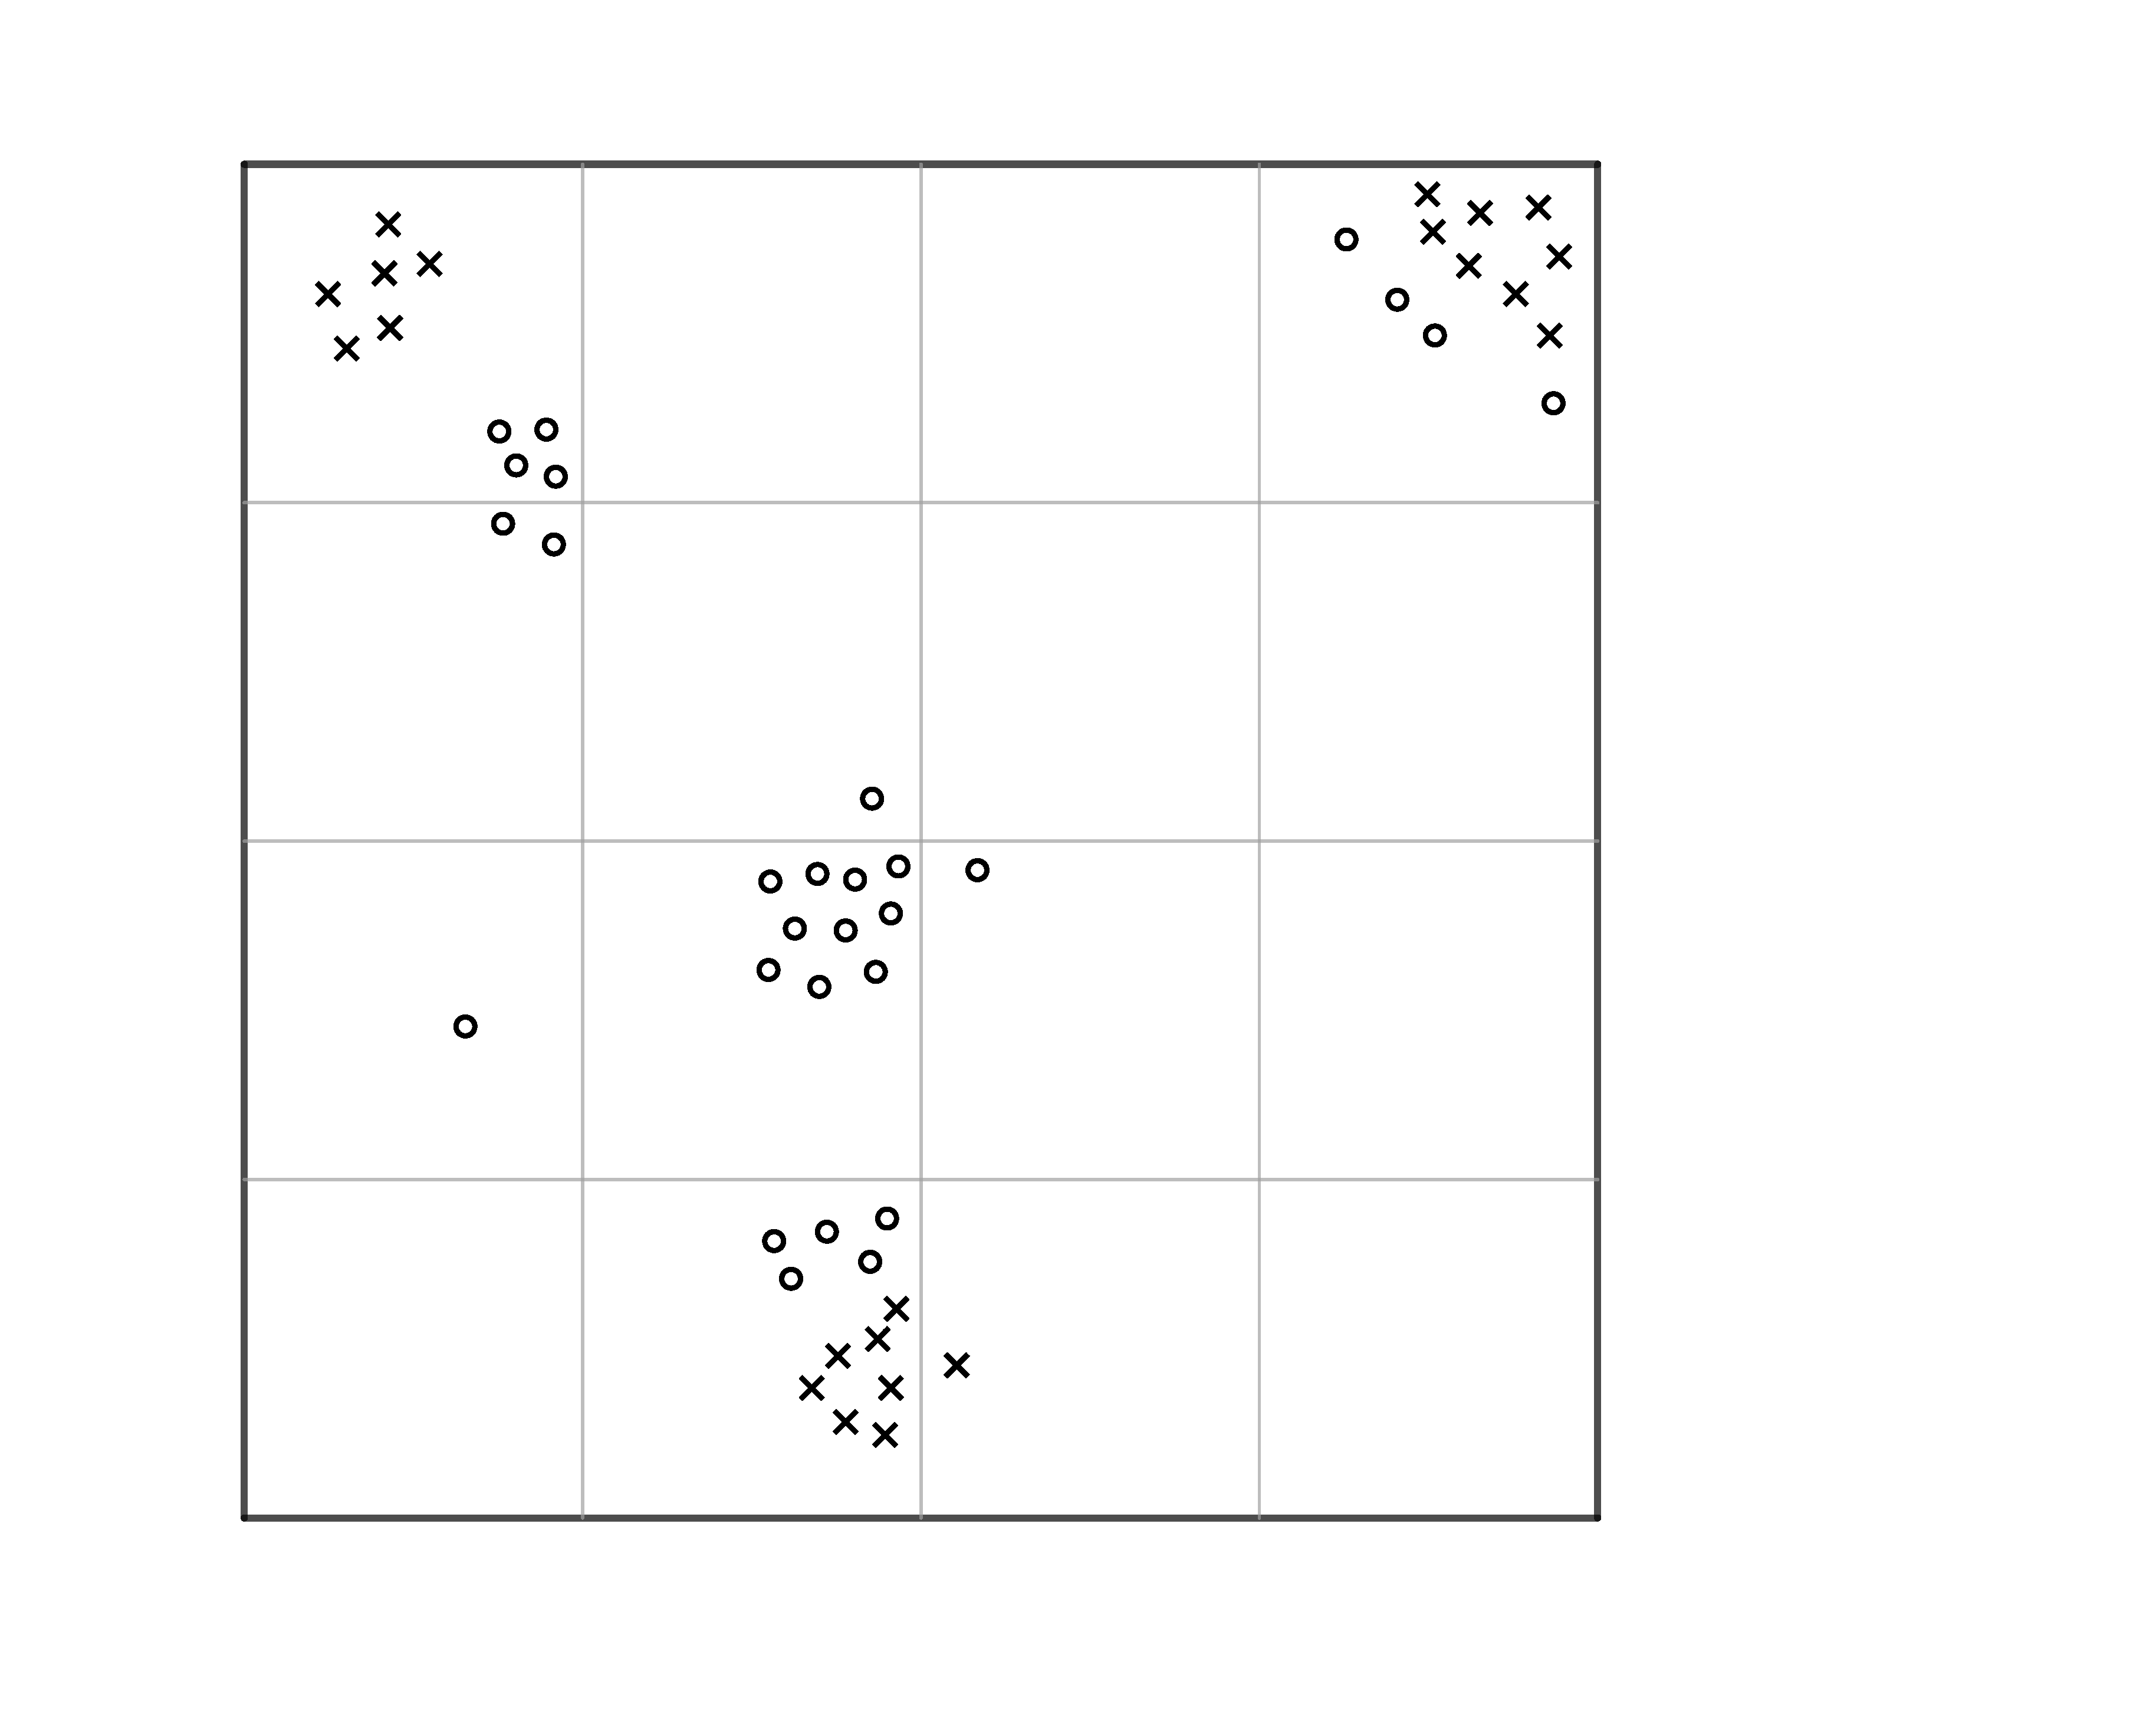
\includegraphics[width=2in]{Gerry4x4-50-2.pdf} &  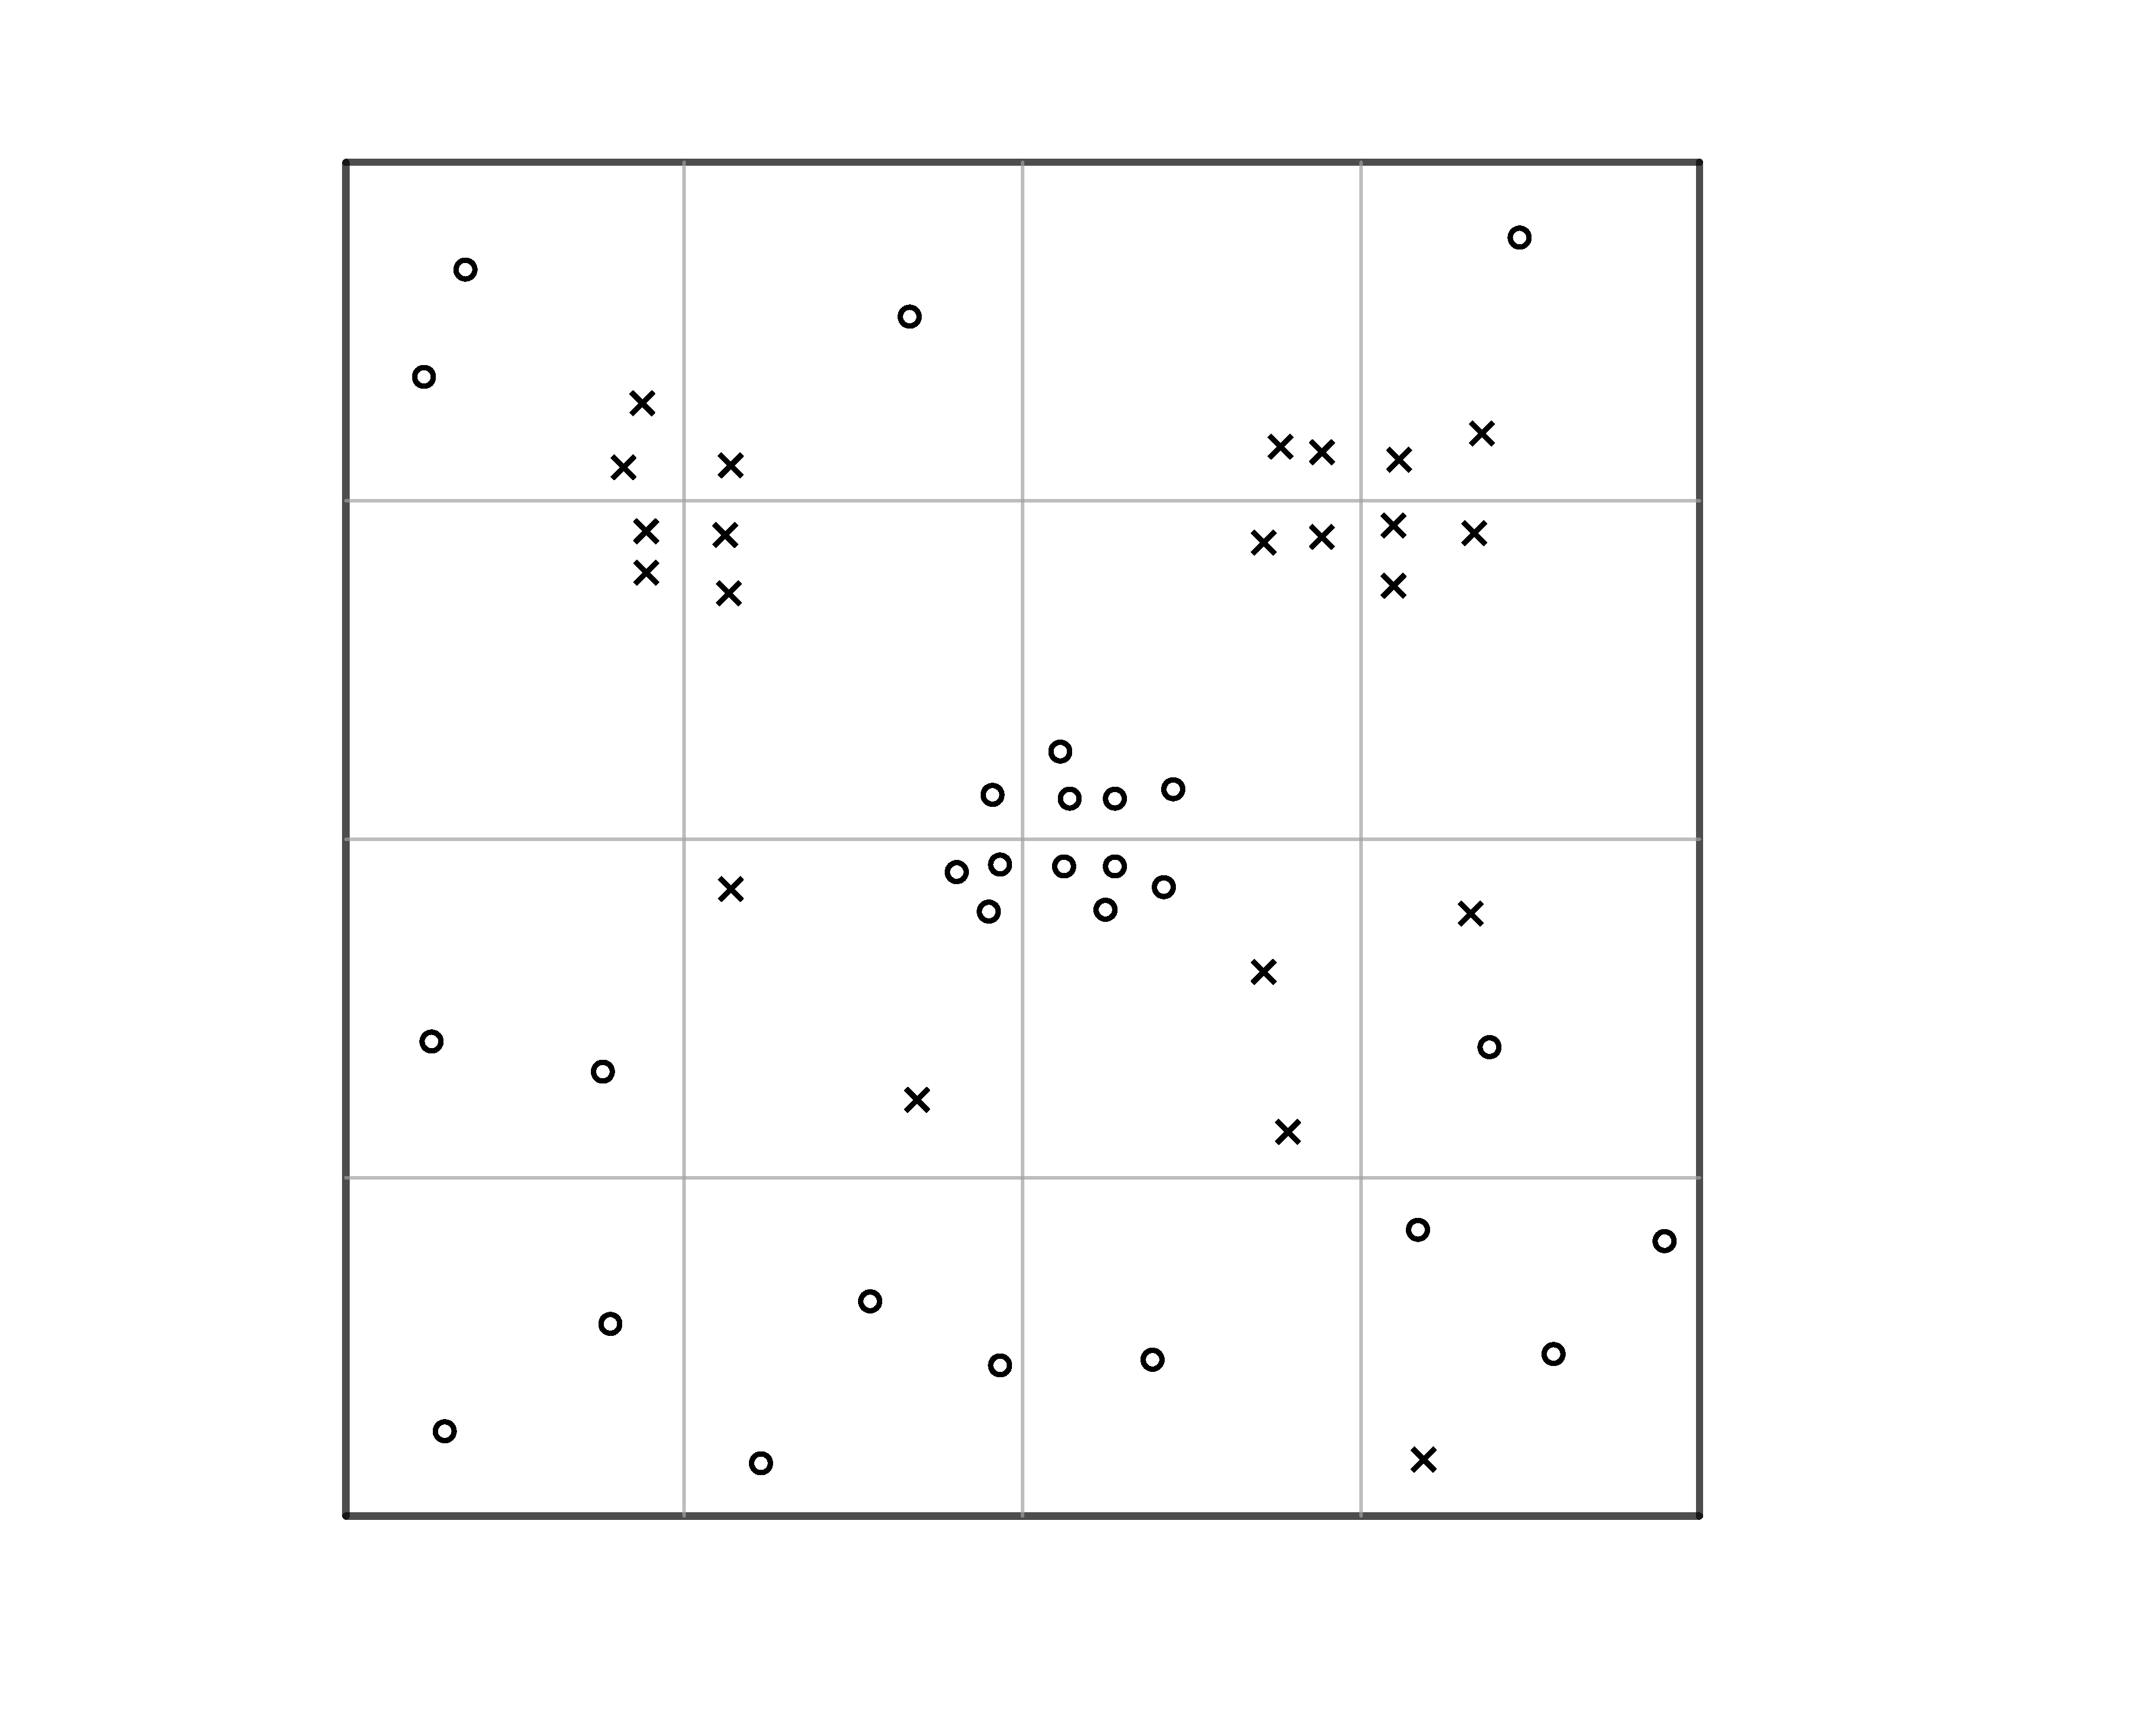
\includegraphics[width=2in]{Gerry4x4-50-3.pdf}\\
 Total Vote Count &  Total Vote Count &  Total Vote Count\\
 X - 22 & X - 22 & X  - 22\\
 O - 28 & O - 28 & O - 28
\end{tabular}



Province B\\
Population = 80
\begin{tabular}{c c c }

Year 1 & Year 2 & Year 3 \\
 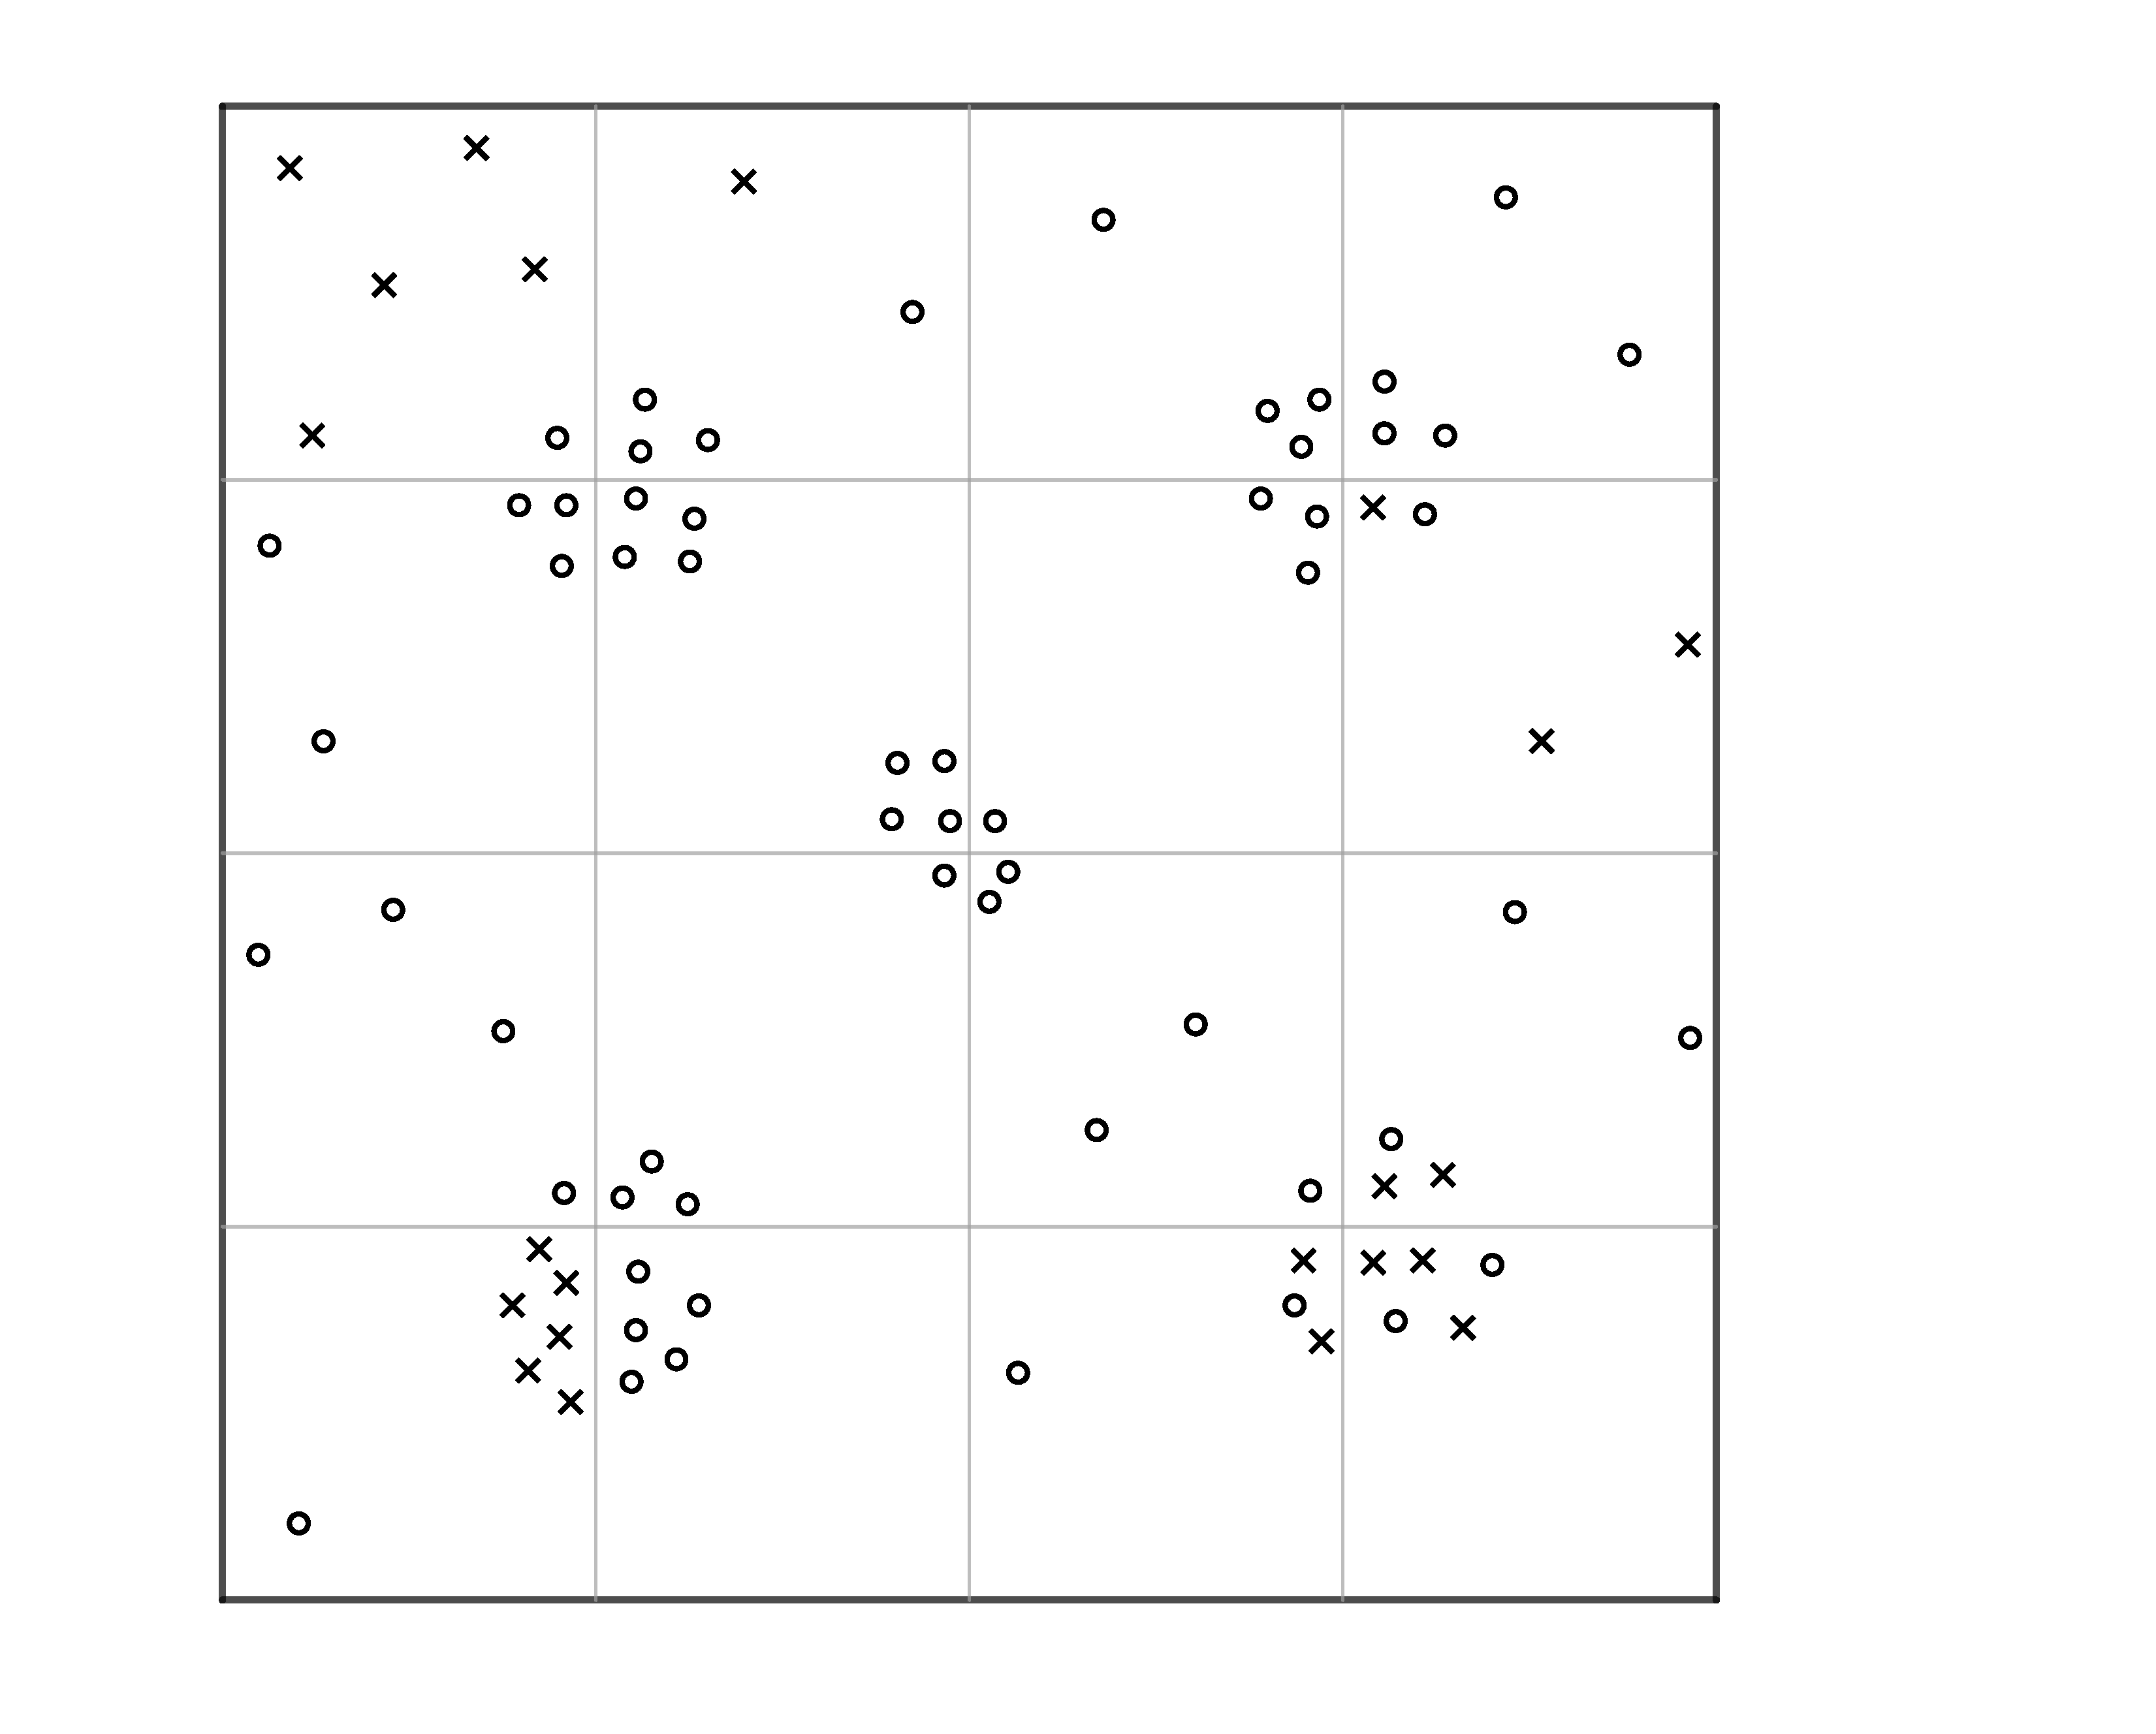
\includegraphics[width=2in]{Gerry4x4-80-1.pdf} &  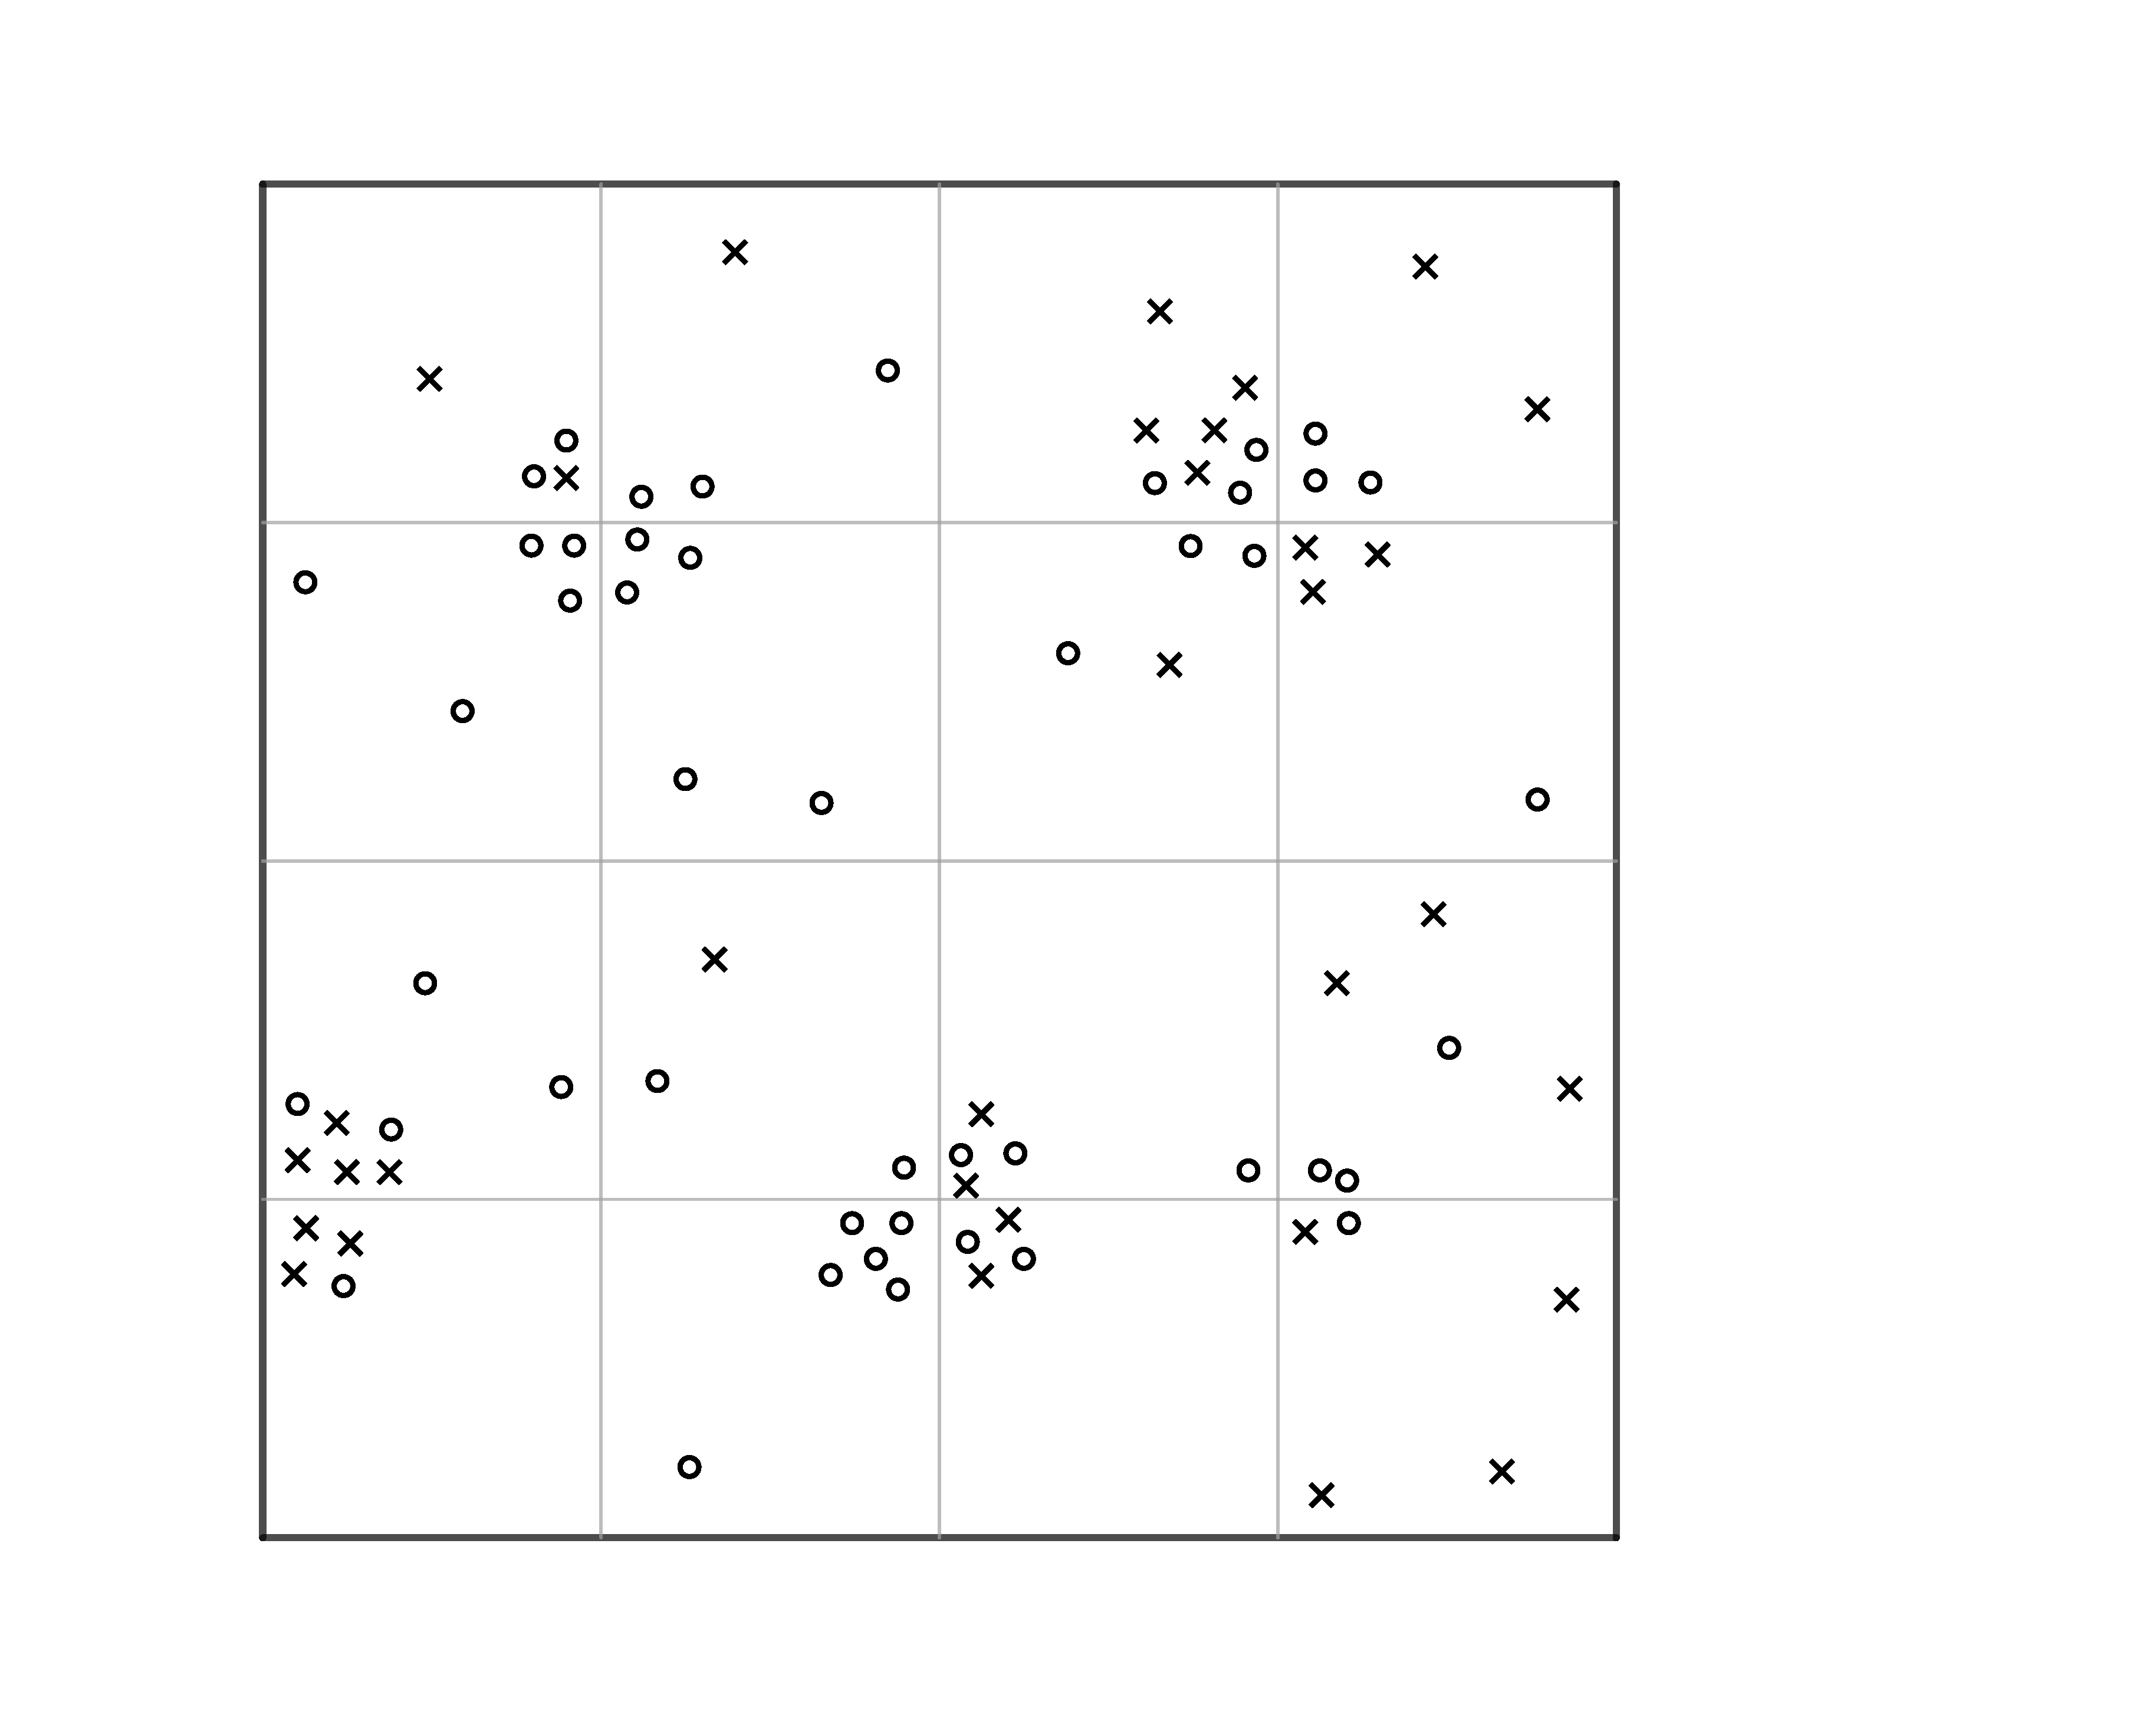
\includegraphics[width=2in]{Gerry4x4-80-2.pdf} &  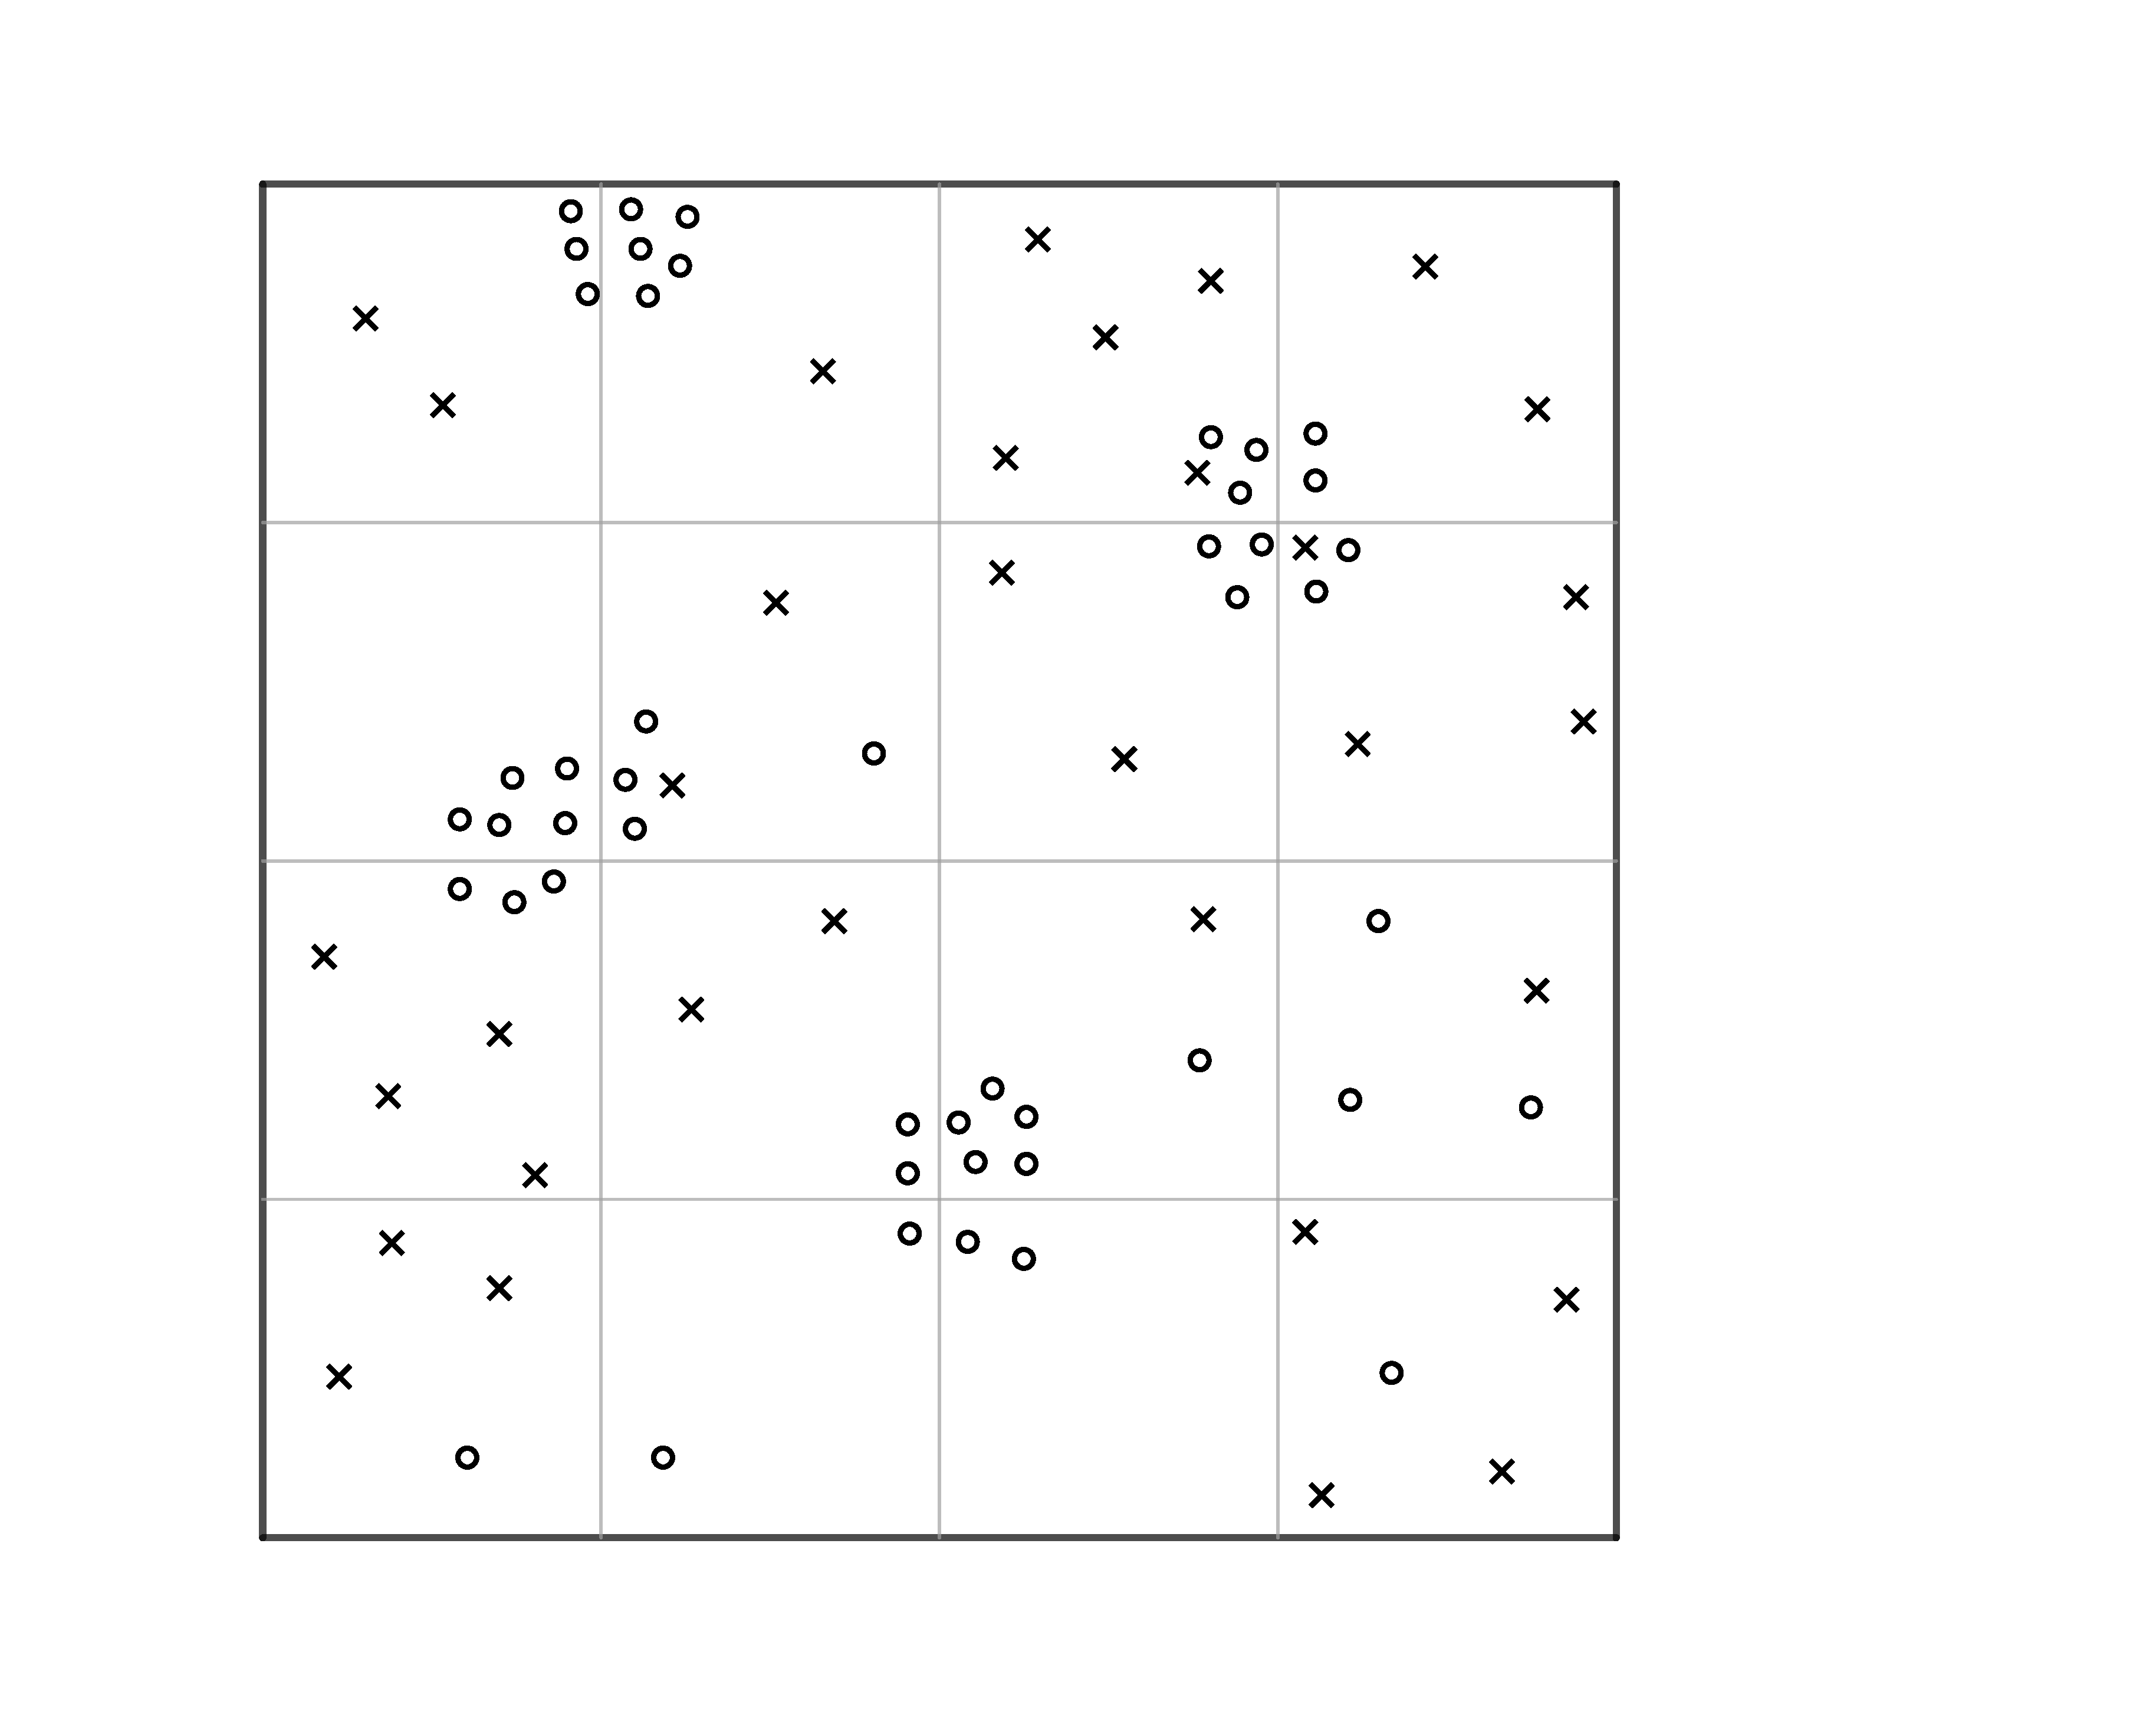
\includegraphics[width=2in]{Gerry4x4-80-3.pdf}\\
 Total Vote Count &  Total Vote Count &  Total Vote Count\\
 X -  22& X - 33 & X  - 33\\
 O - 58 & O - 47 & O - 47
 \end{tabular}


Province C\\
Population = 100
\begin{tabular}{c c c }

Year 1 & Year 2 & Year 3 \\
 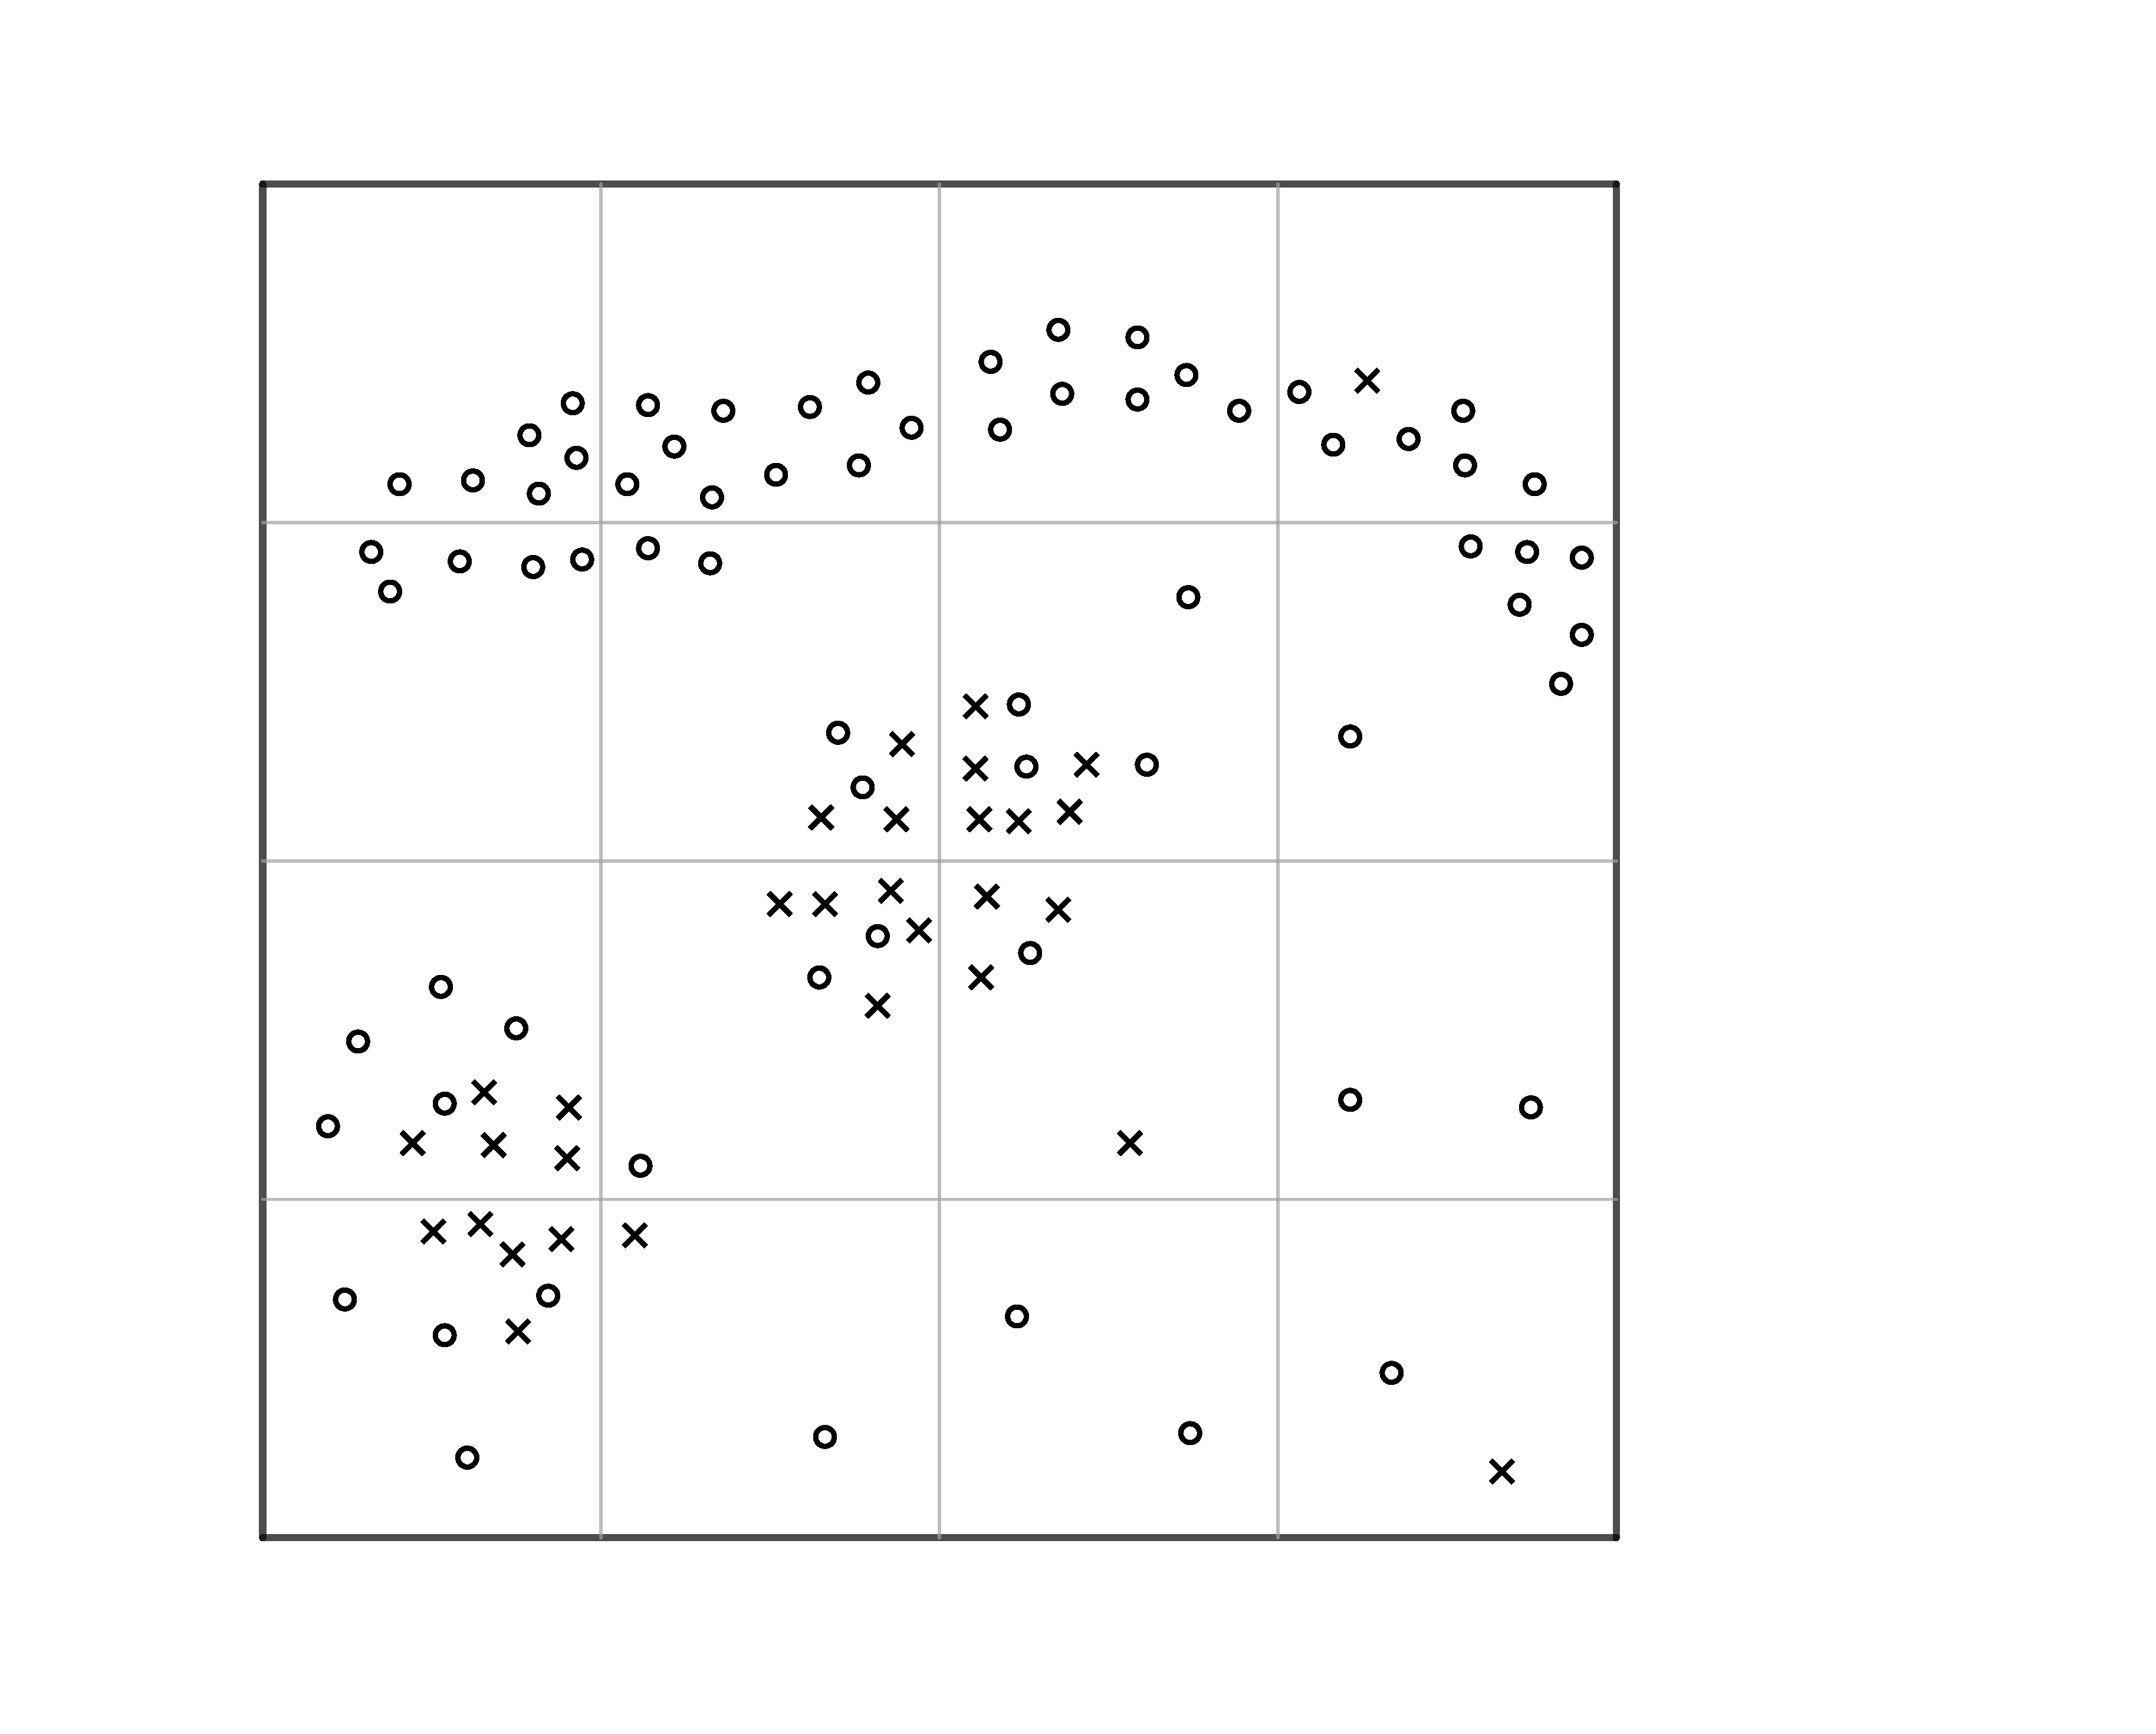
\includegraphics[width=2in]{Gerry4x4-100-1.pdf} &  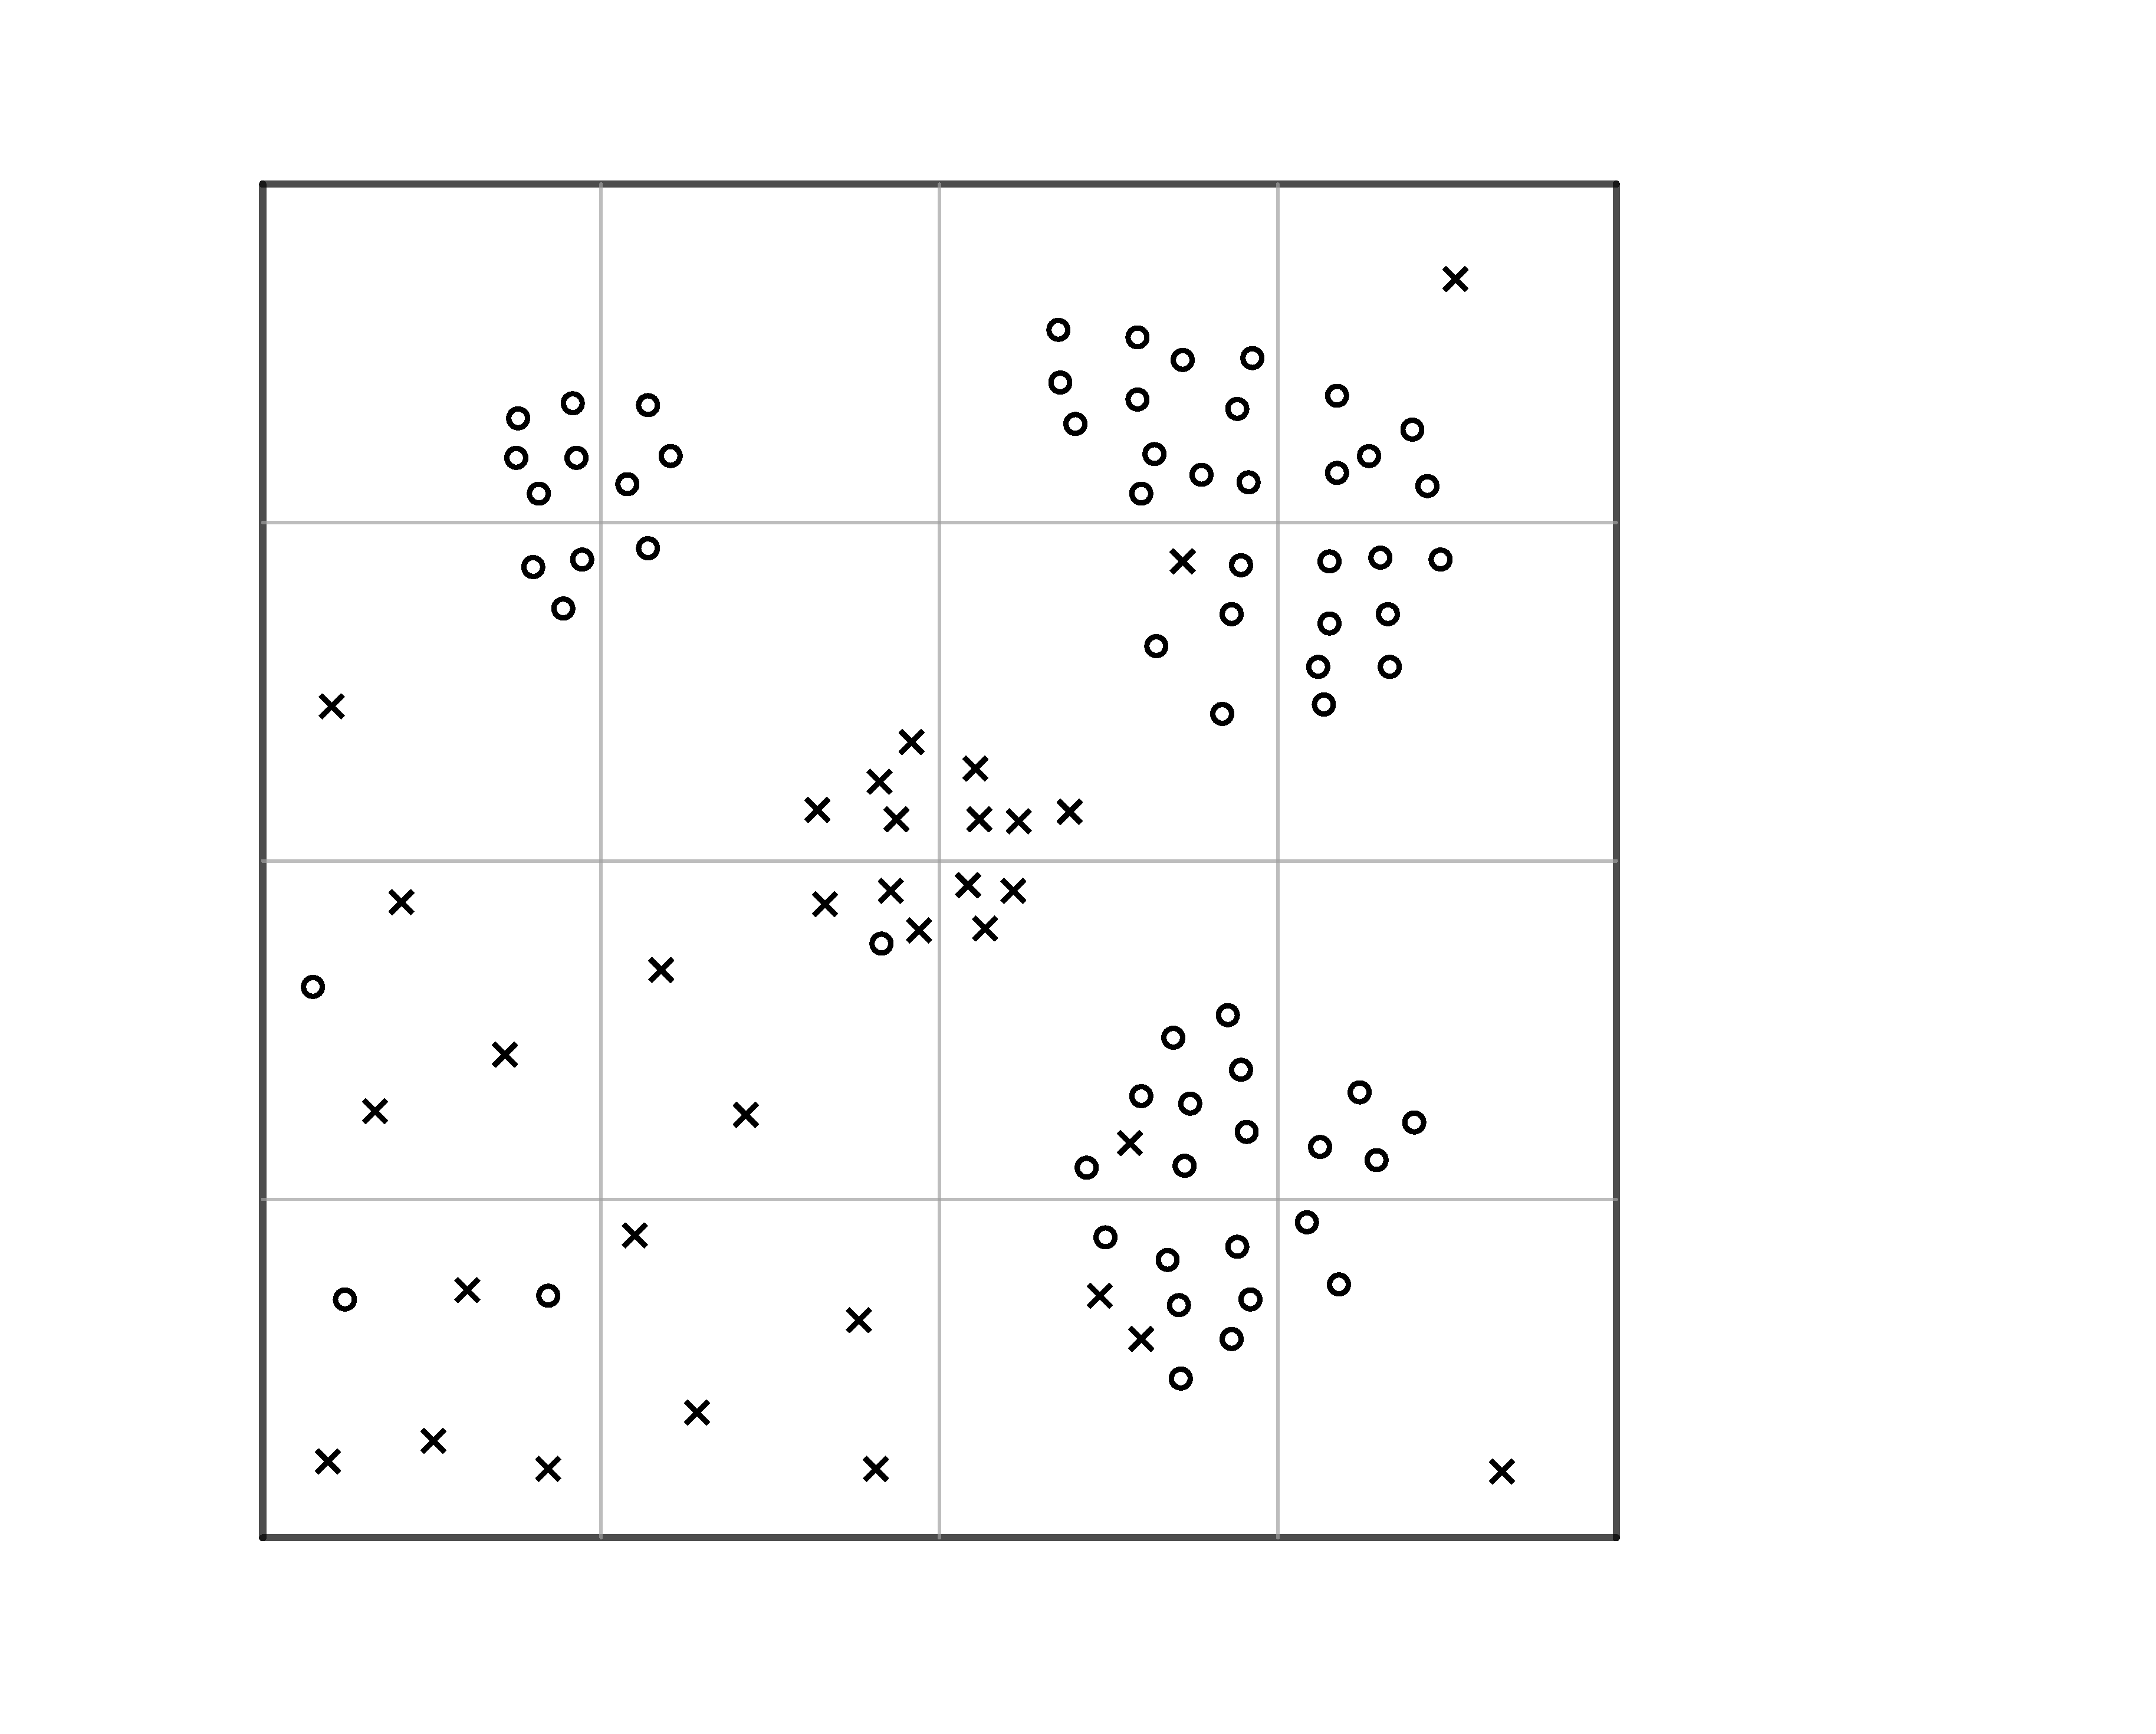
\includegraphics[width=2in]{Gerry4x4-100-2.pdf} &  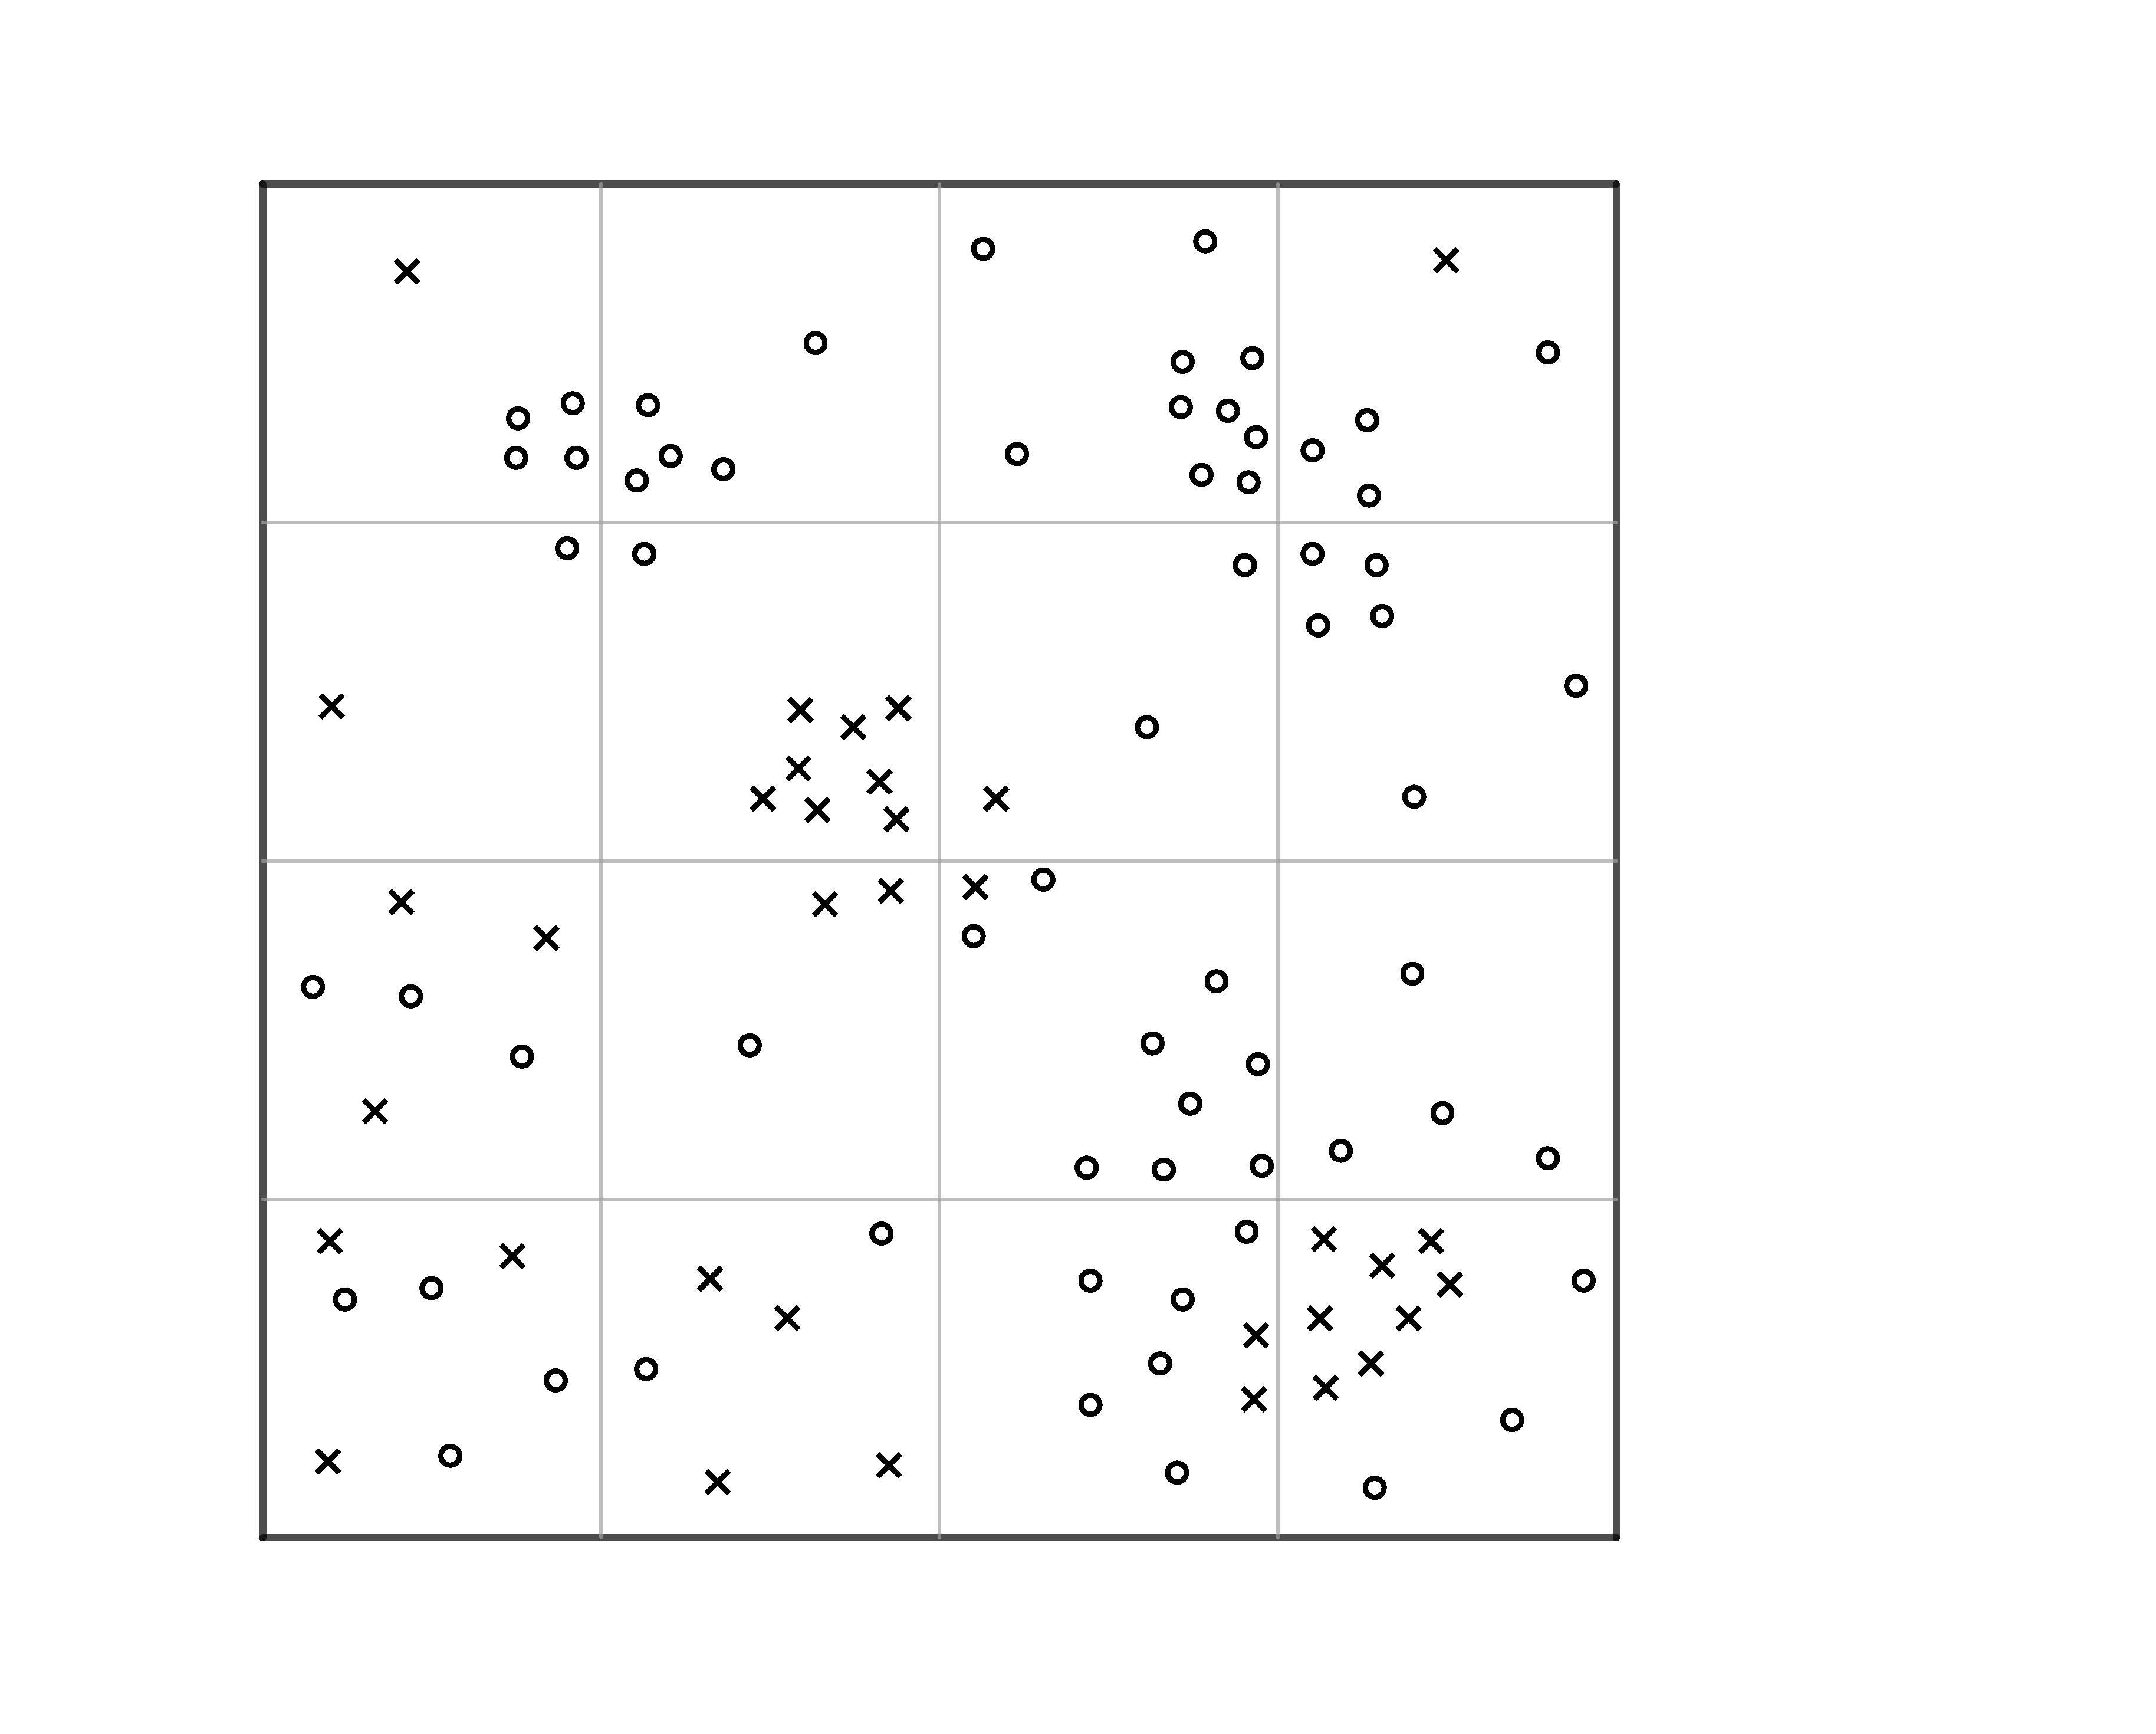
\includegraphics[width=2in]{Gerry4x4-100-3.pdf}\\
 Total Vote Count &  Total Vote Count &  Total Vote Count\\
 X -  31& X - 34 & X  - 35\\
 O - 69 & O - 66 & O - 65
 \end{tabular}
\newpage


Province D\\
Population = 100
\begin{tabular}{c c c }

Year 1 & Year 2 & Year 3 \\
 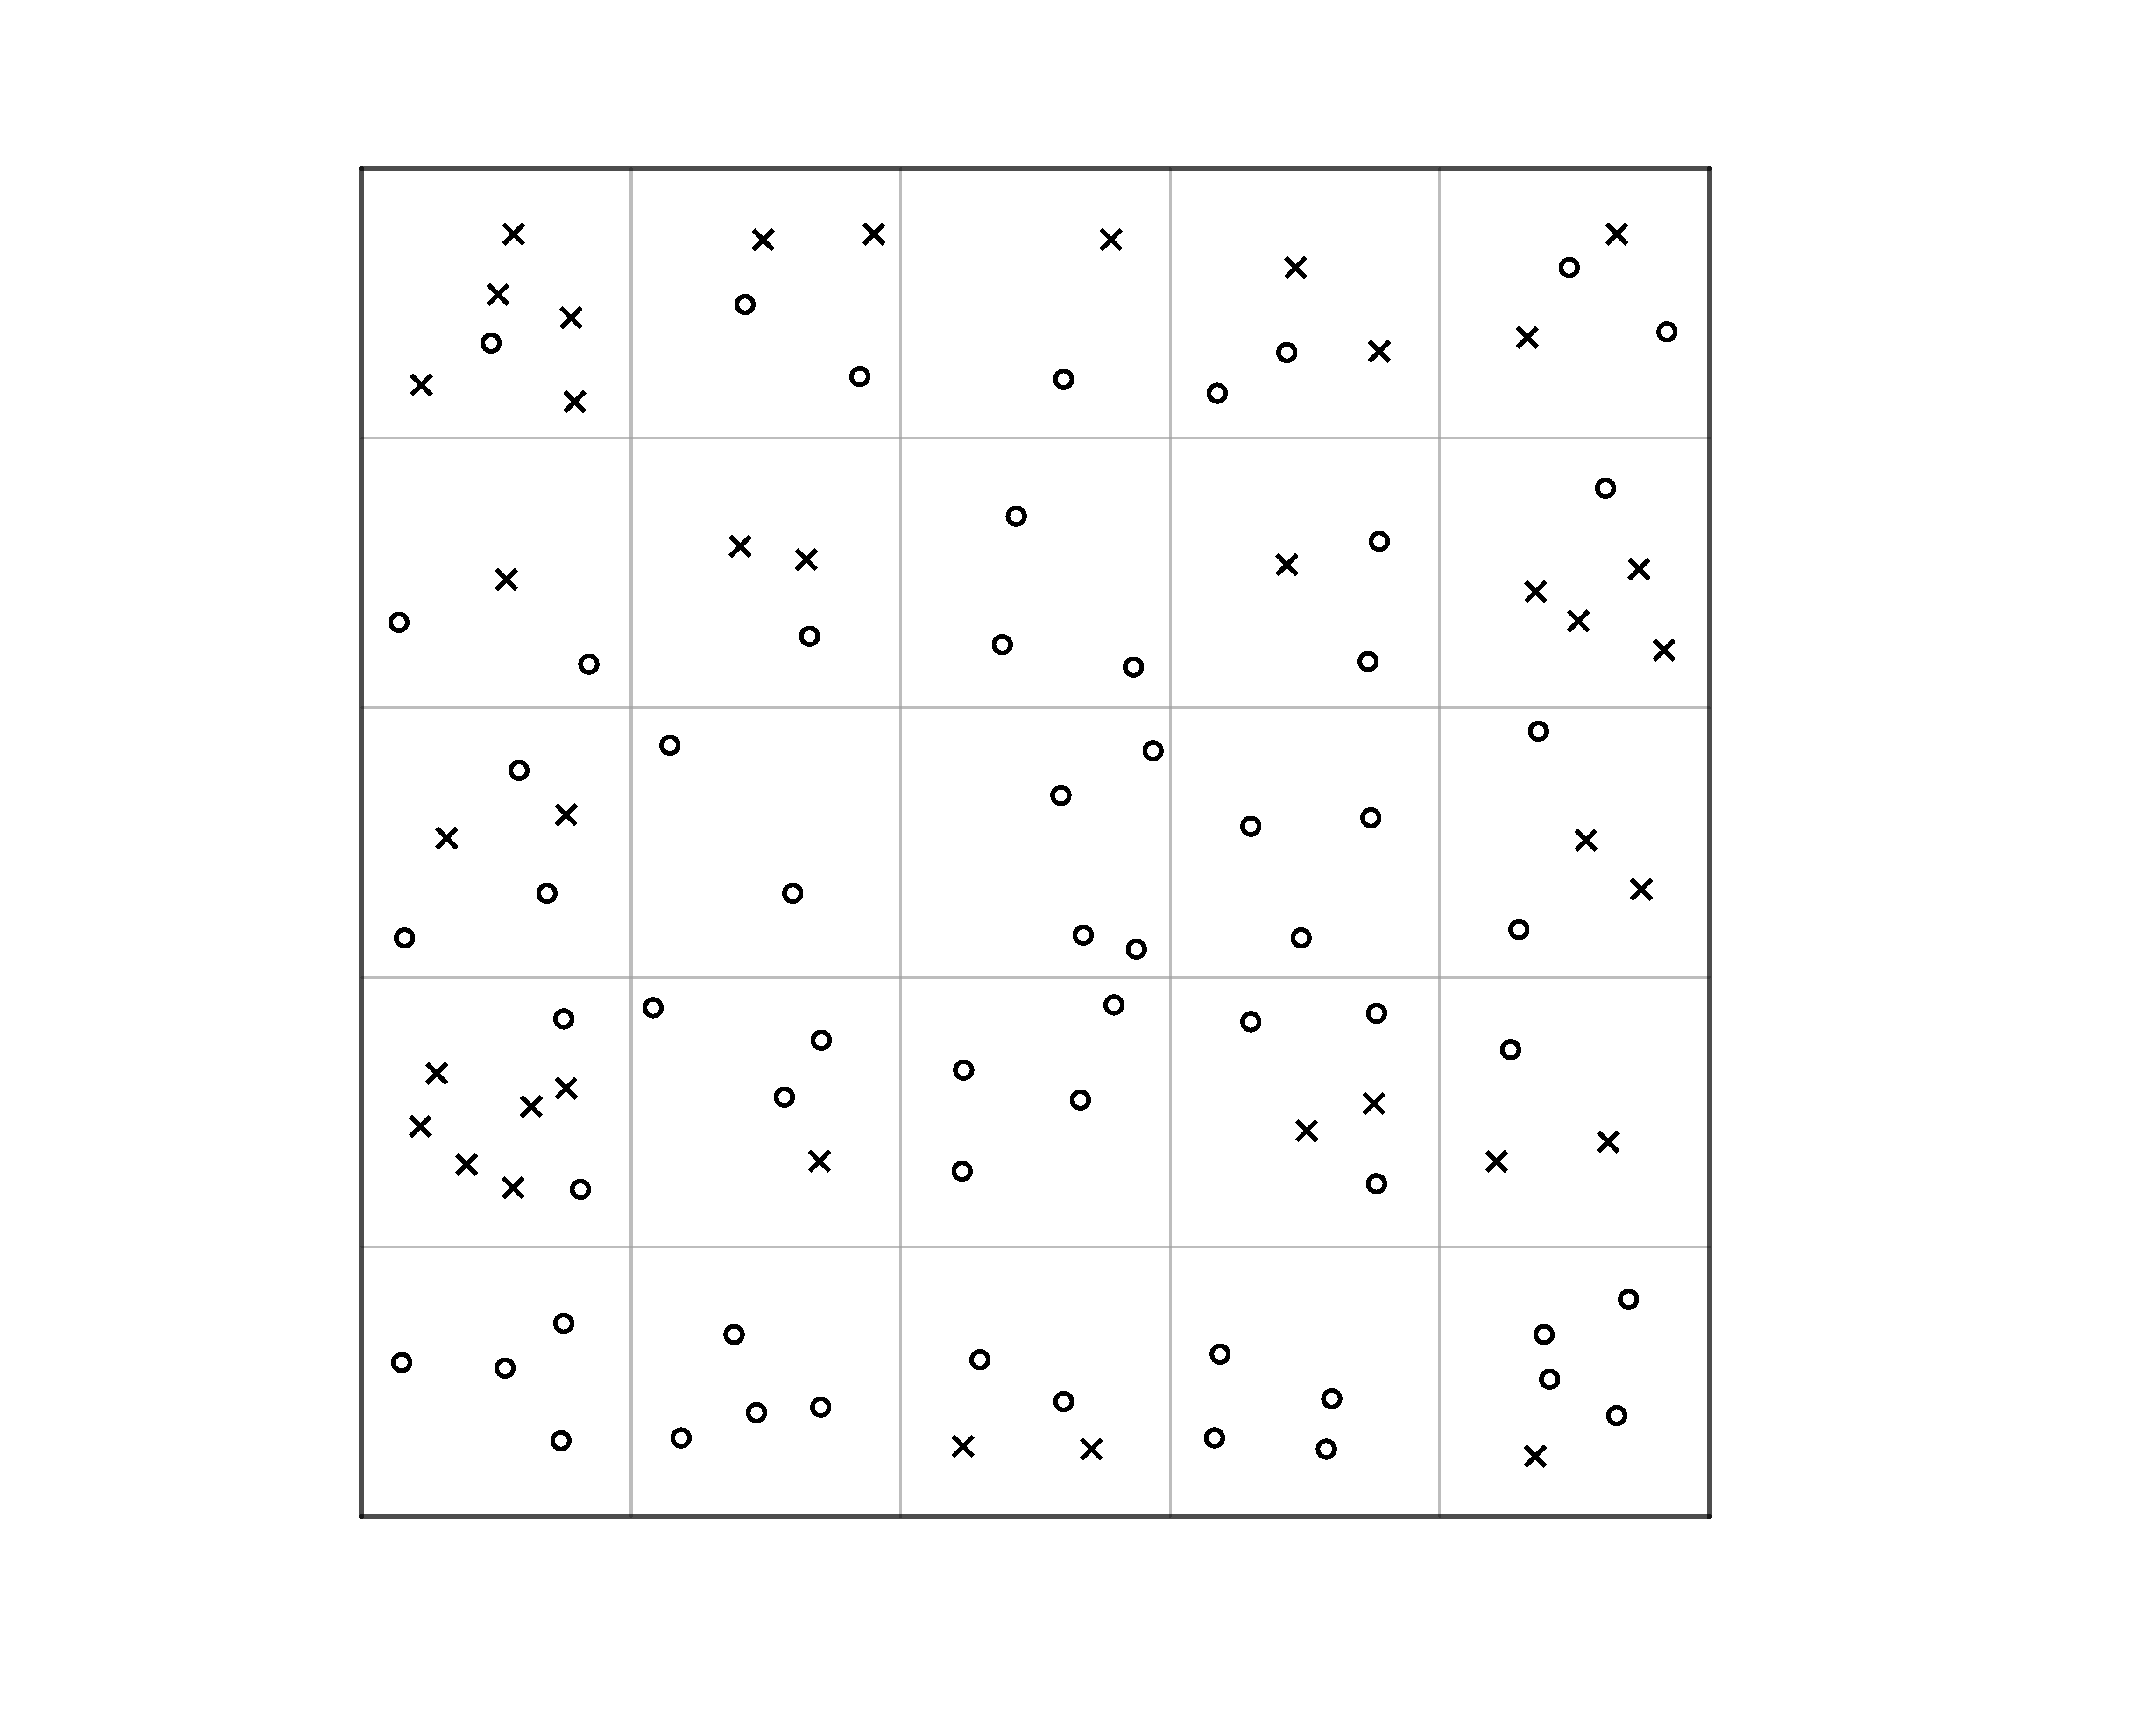
\includegraphics[width=2in]{Gerry5x5-100-1.pdf} &  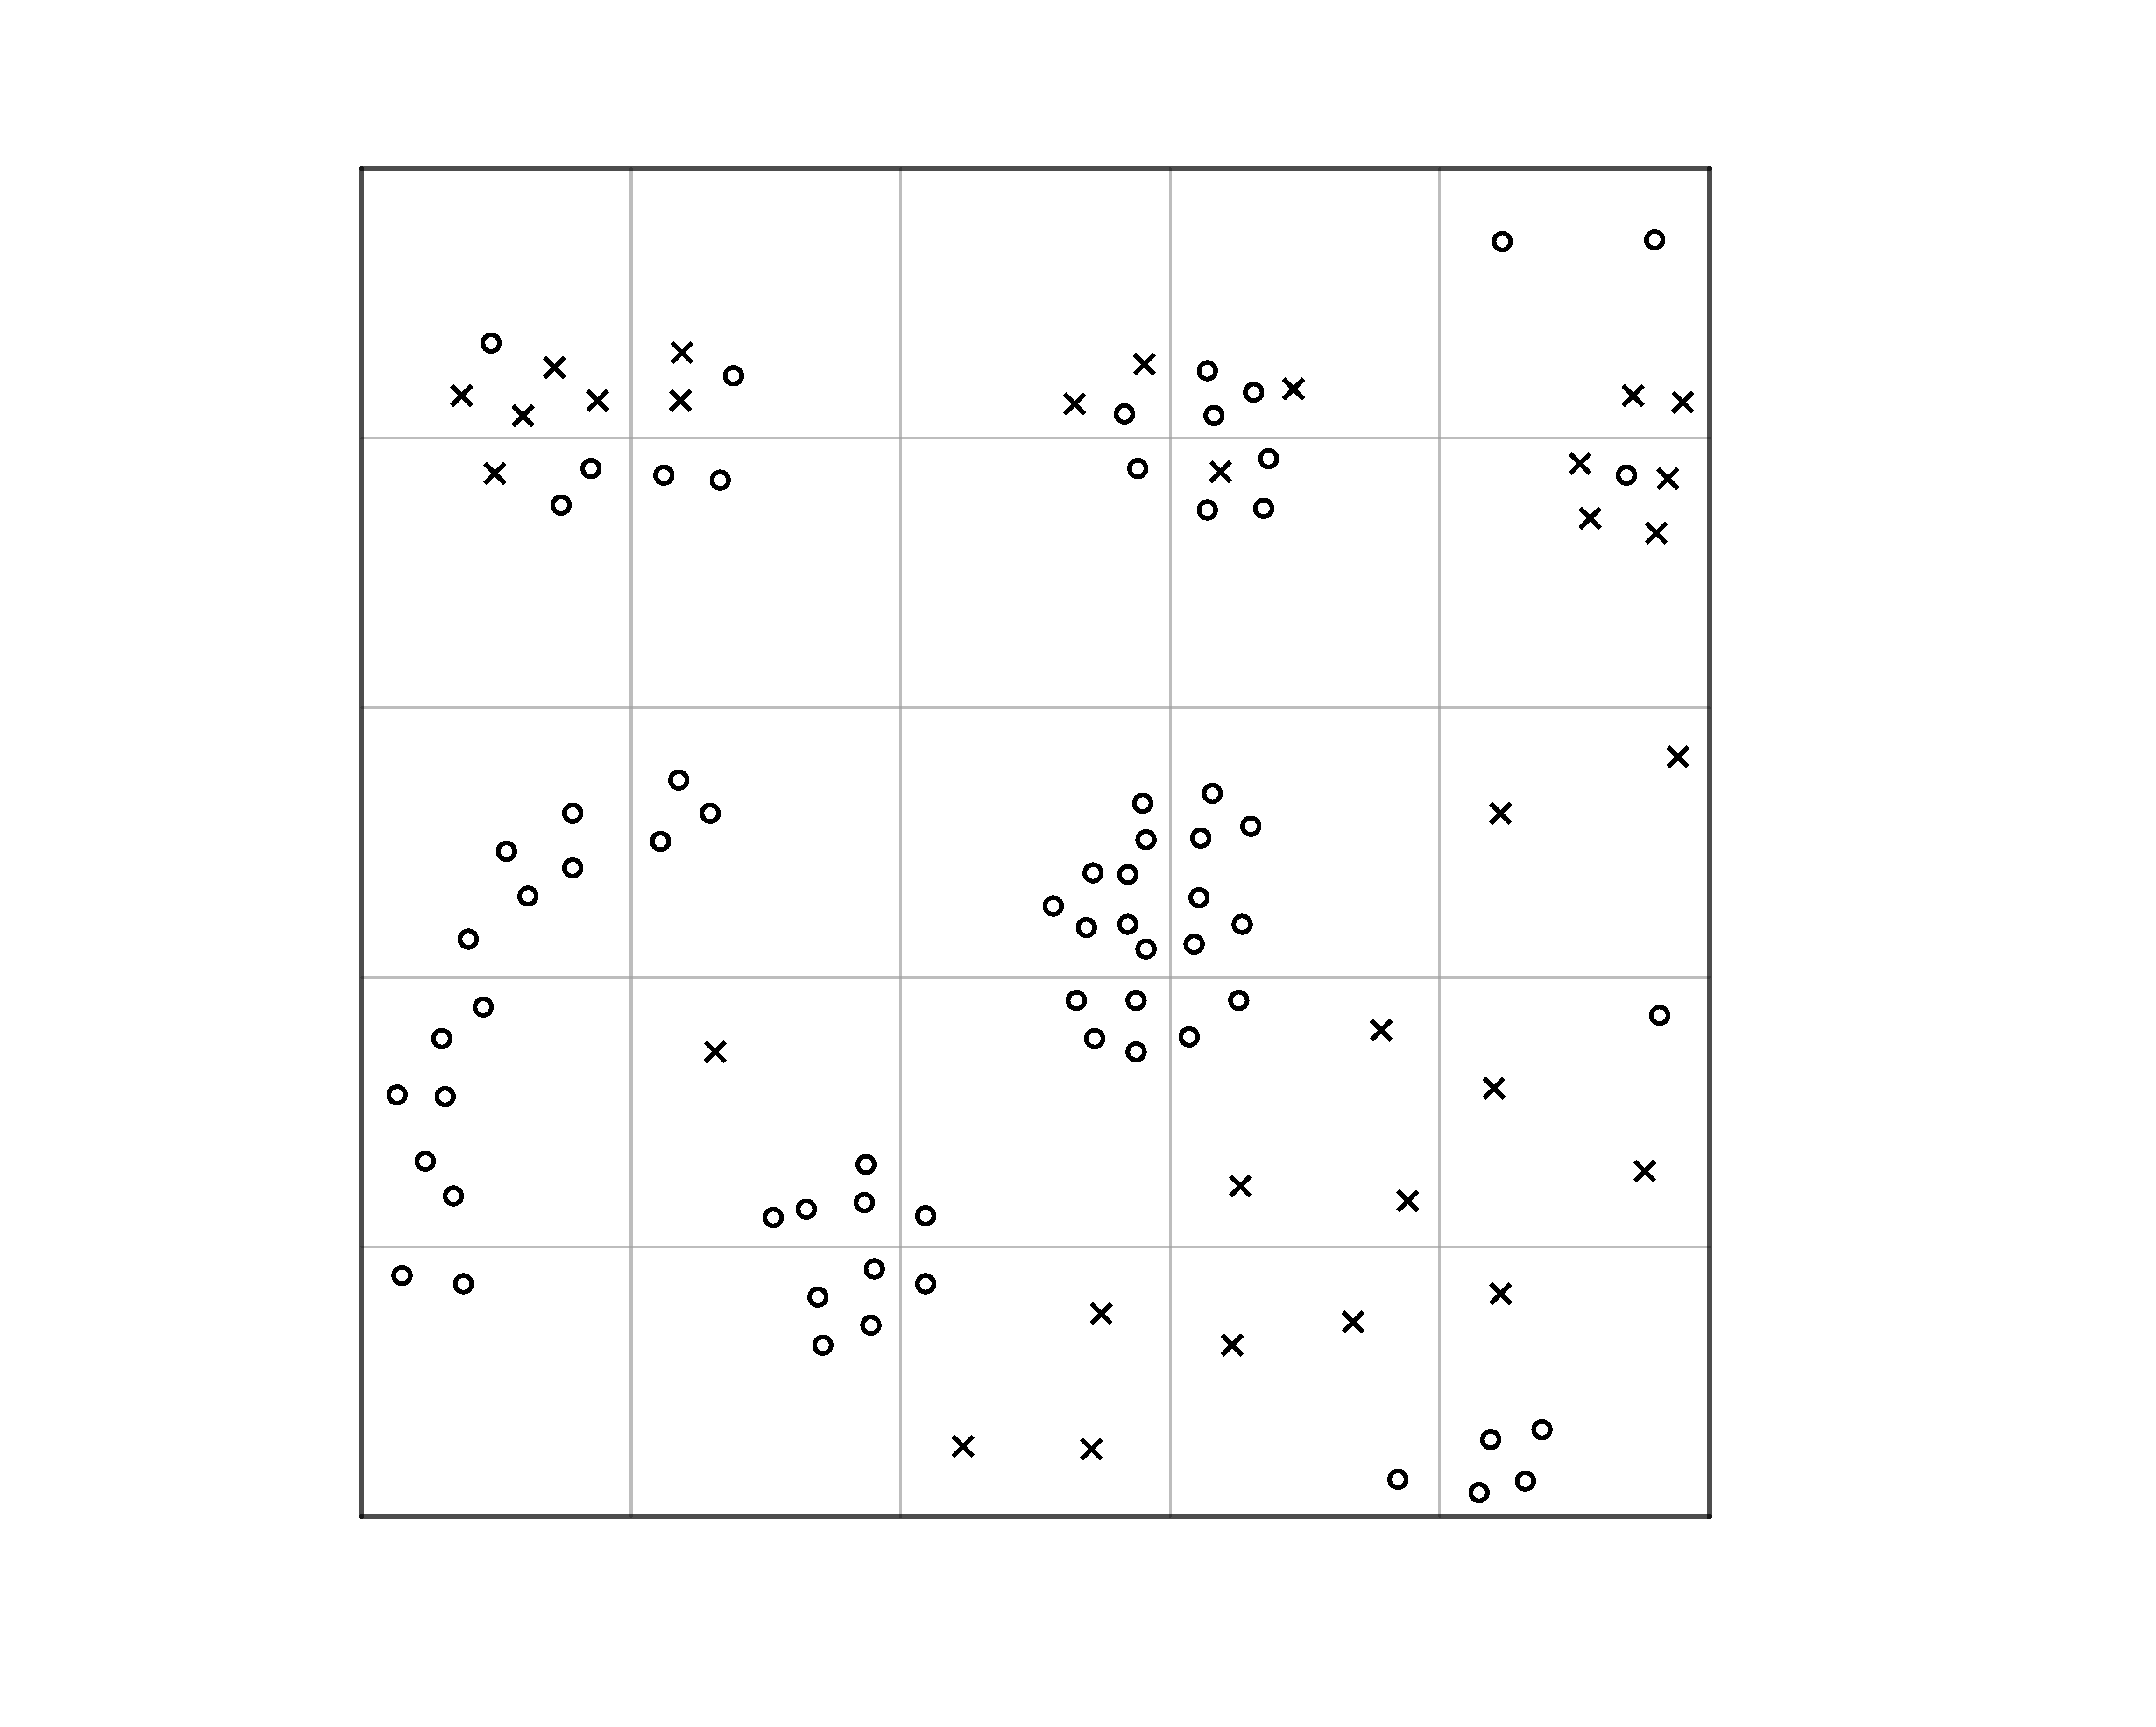
\includegraphics[width=2in]{Gerry5x5-100-2.pdf} &  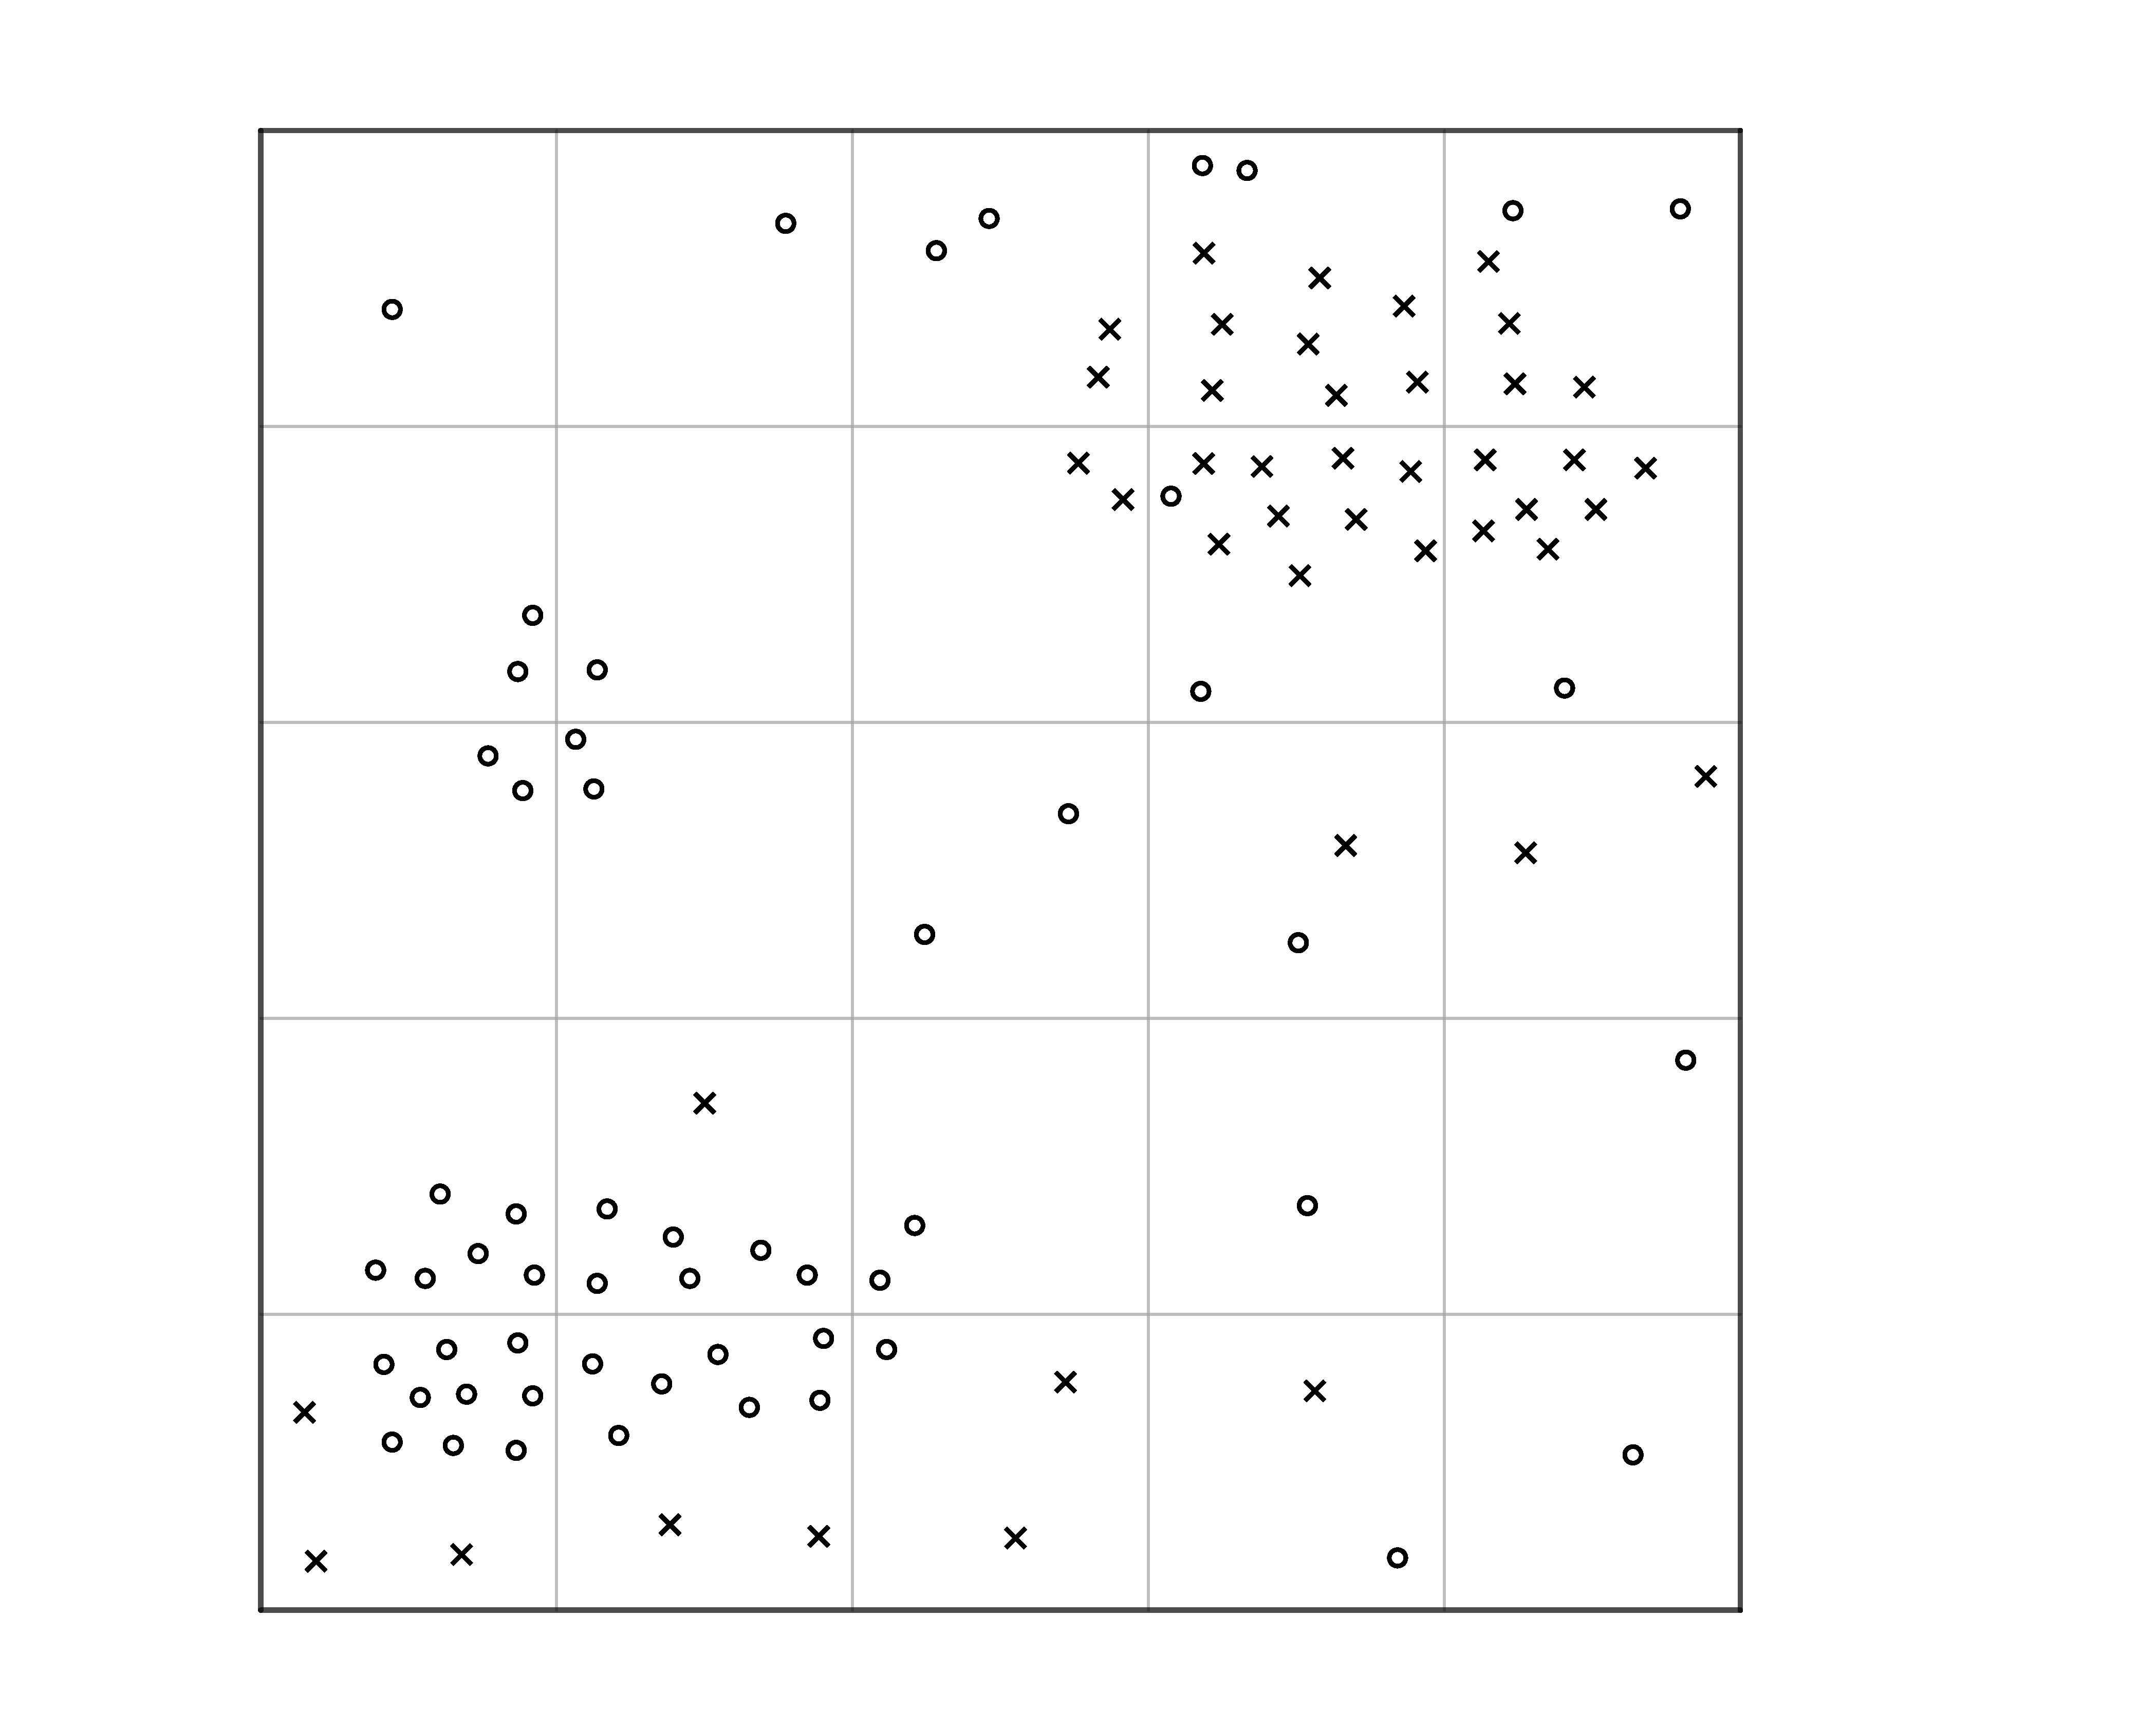
\includegraphics[width=2in]{Gerry5x5-100-3.pdf}\\
 Total Vote Count &  Total Vote Count &  Total Vote Count\\
 X -  38& X - 31 & X  - 44\\
 O - 62 & O - 69 & O - 56
 \end{tabular}


Province E\\
Population = 120
\begin{tabular}{c c c }

Year 1 & Year 2 & Year 3 \\
 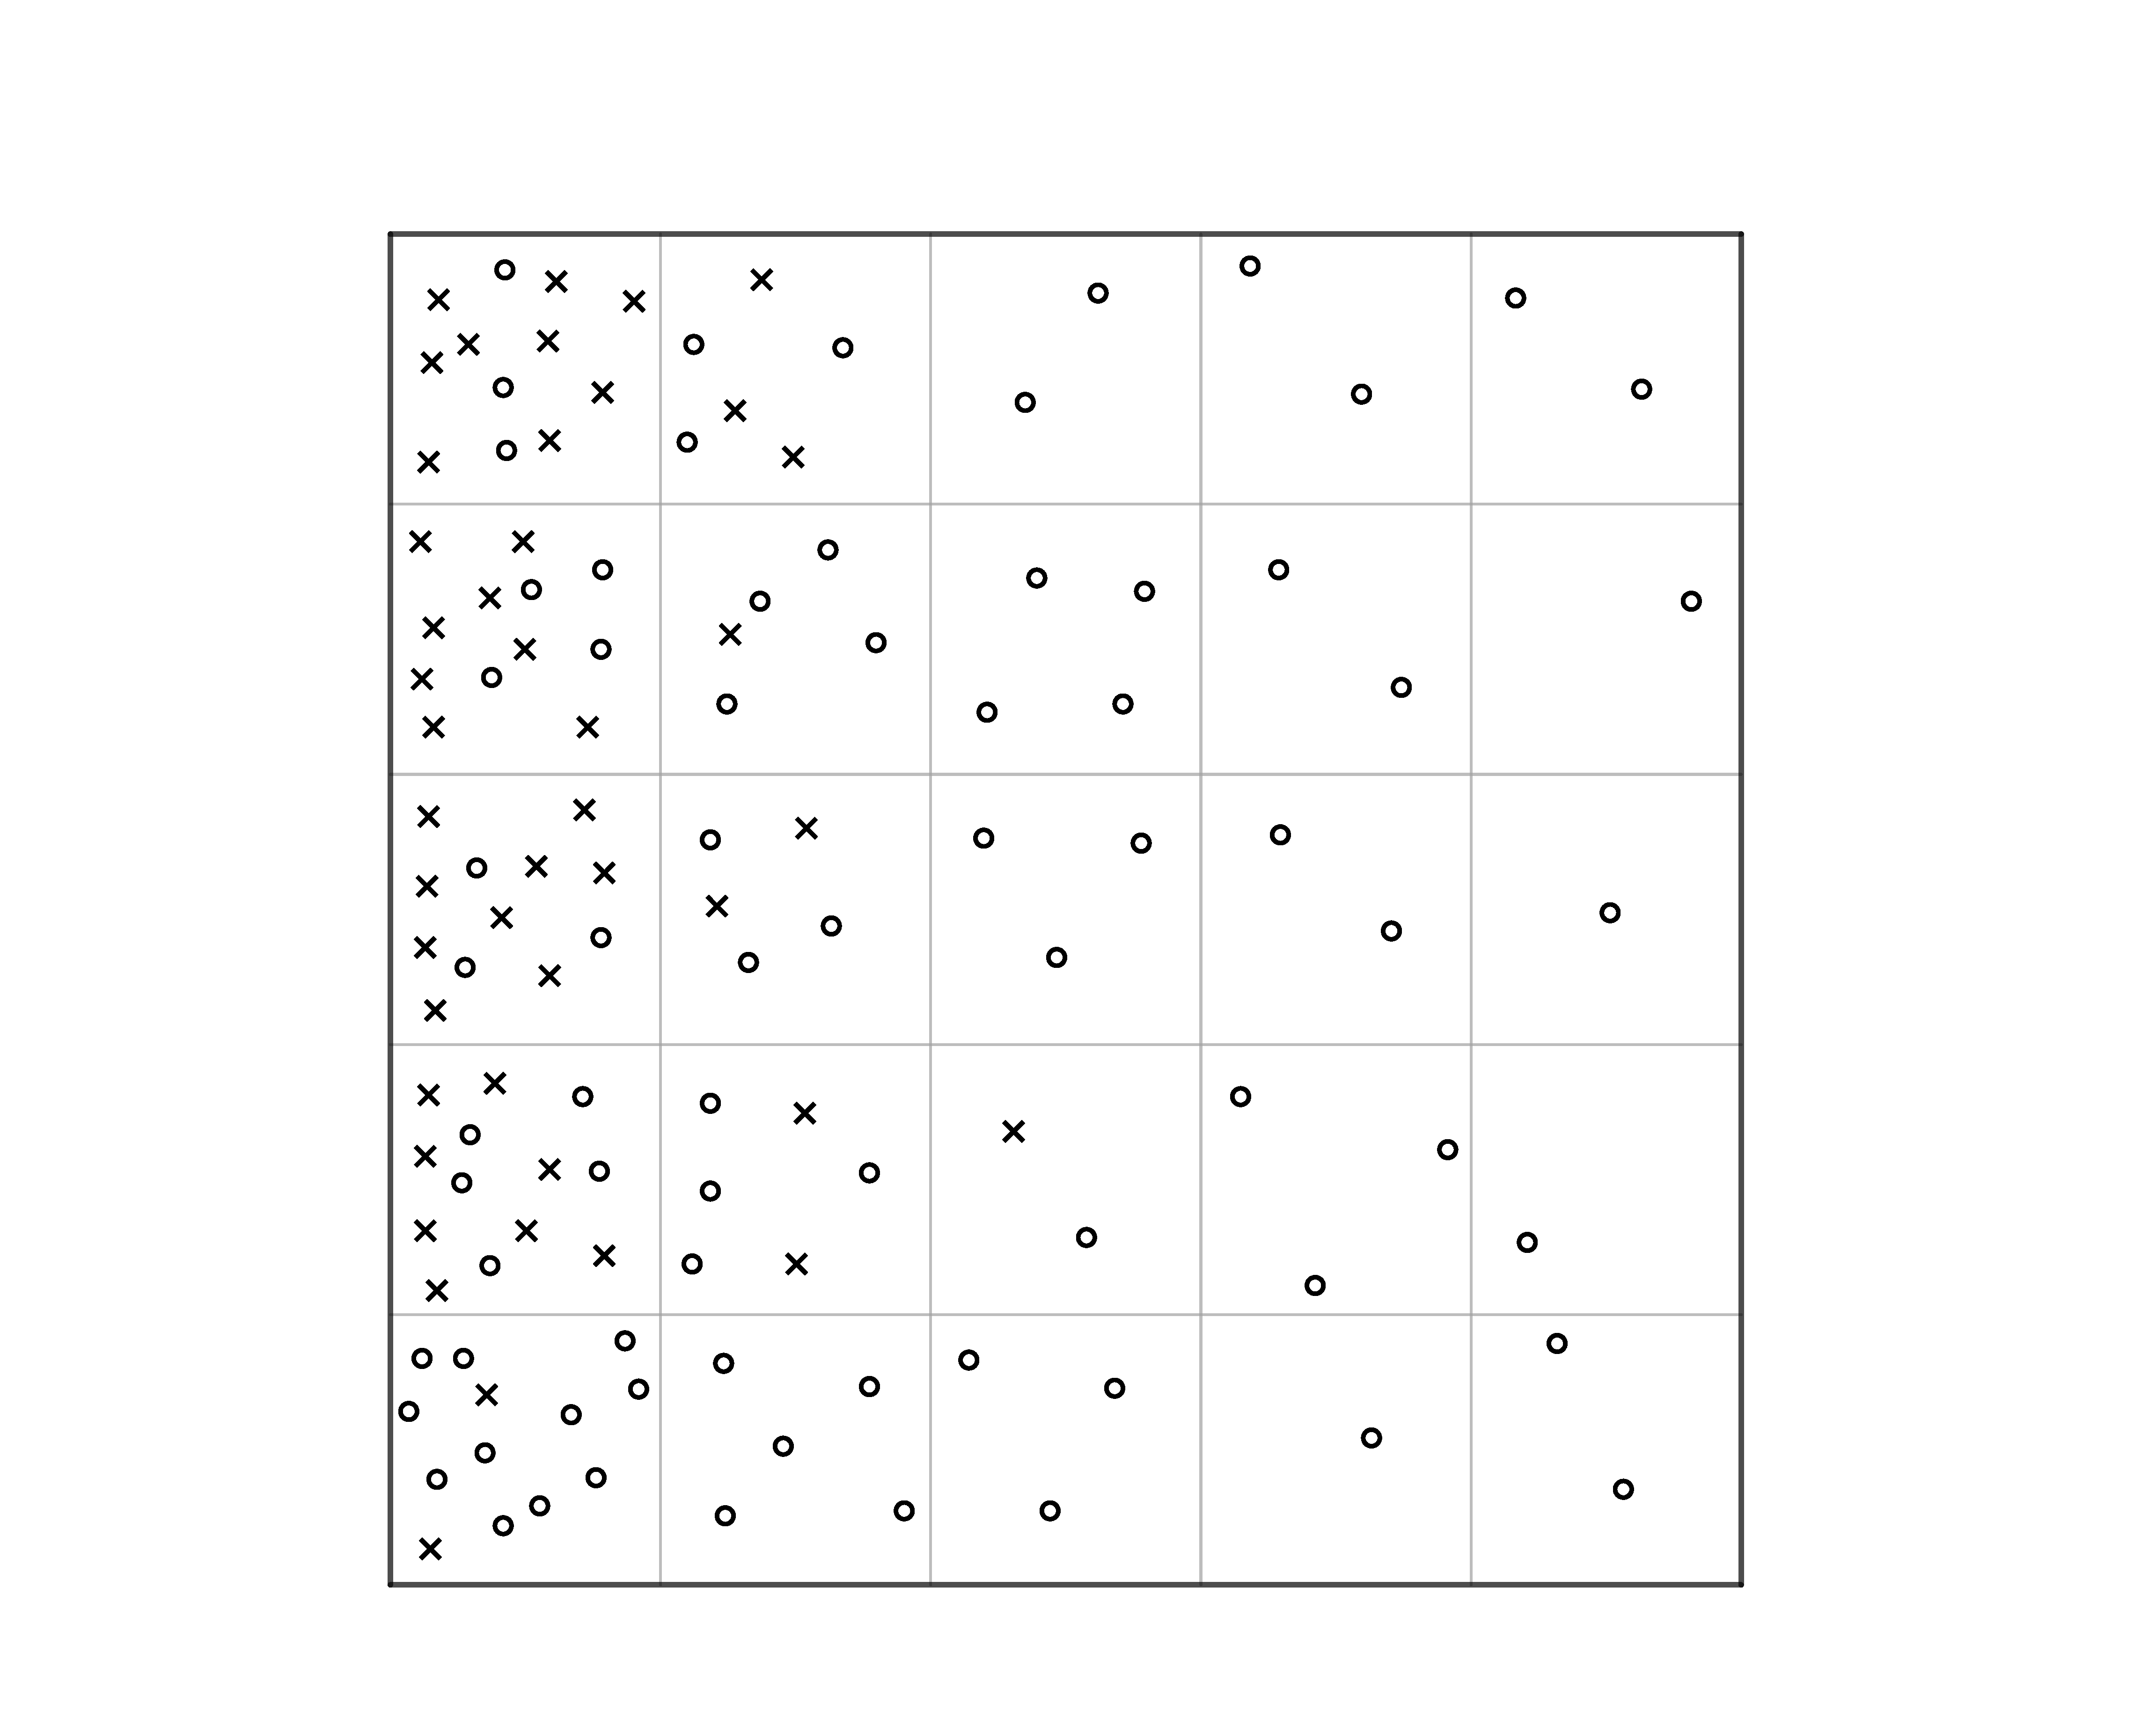
\includegraphics[width=2in]{Gerry5x5-120-1.pdf} &  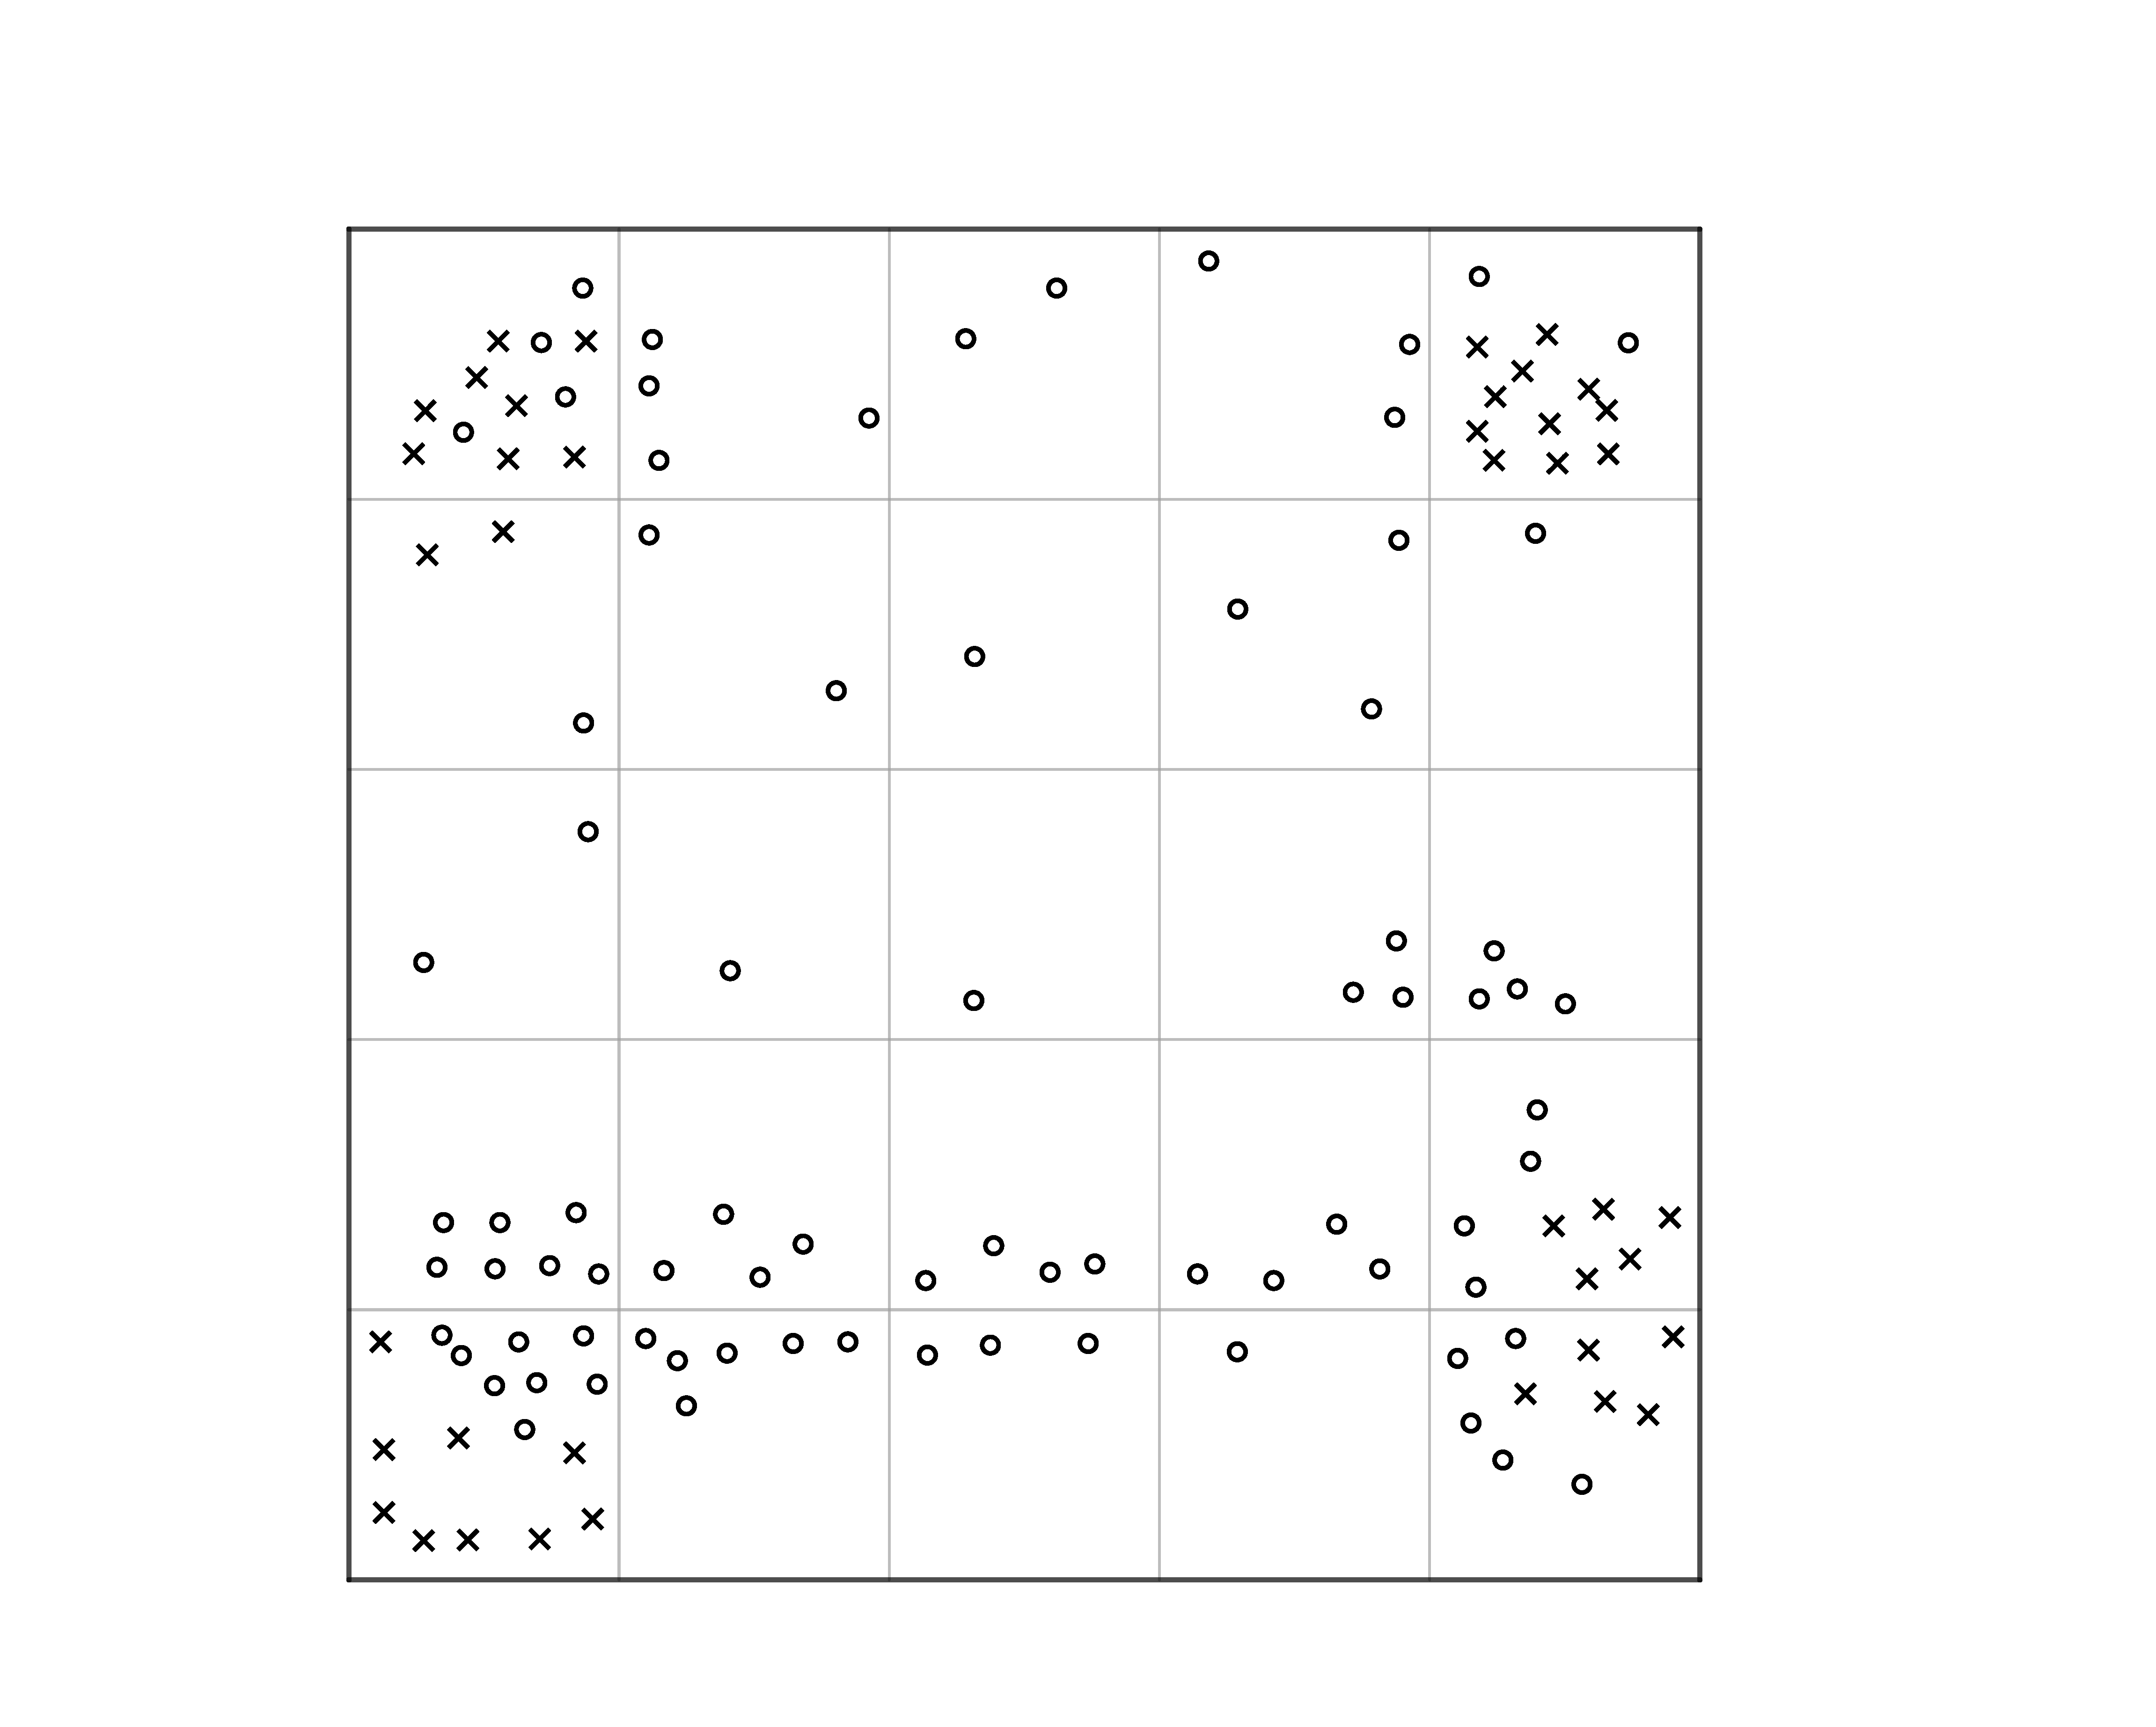
\includegraphics[width=2in]{Gerry5x5-120-2.pdf} &  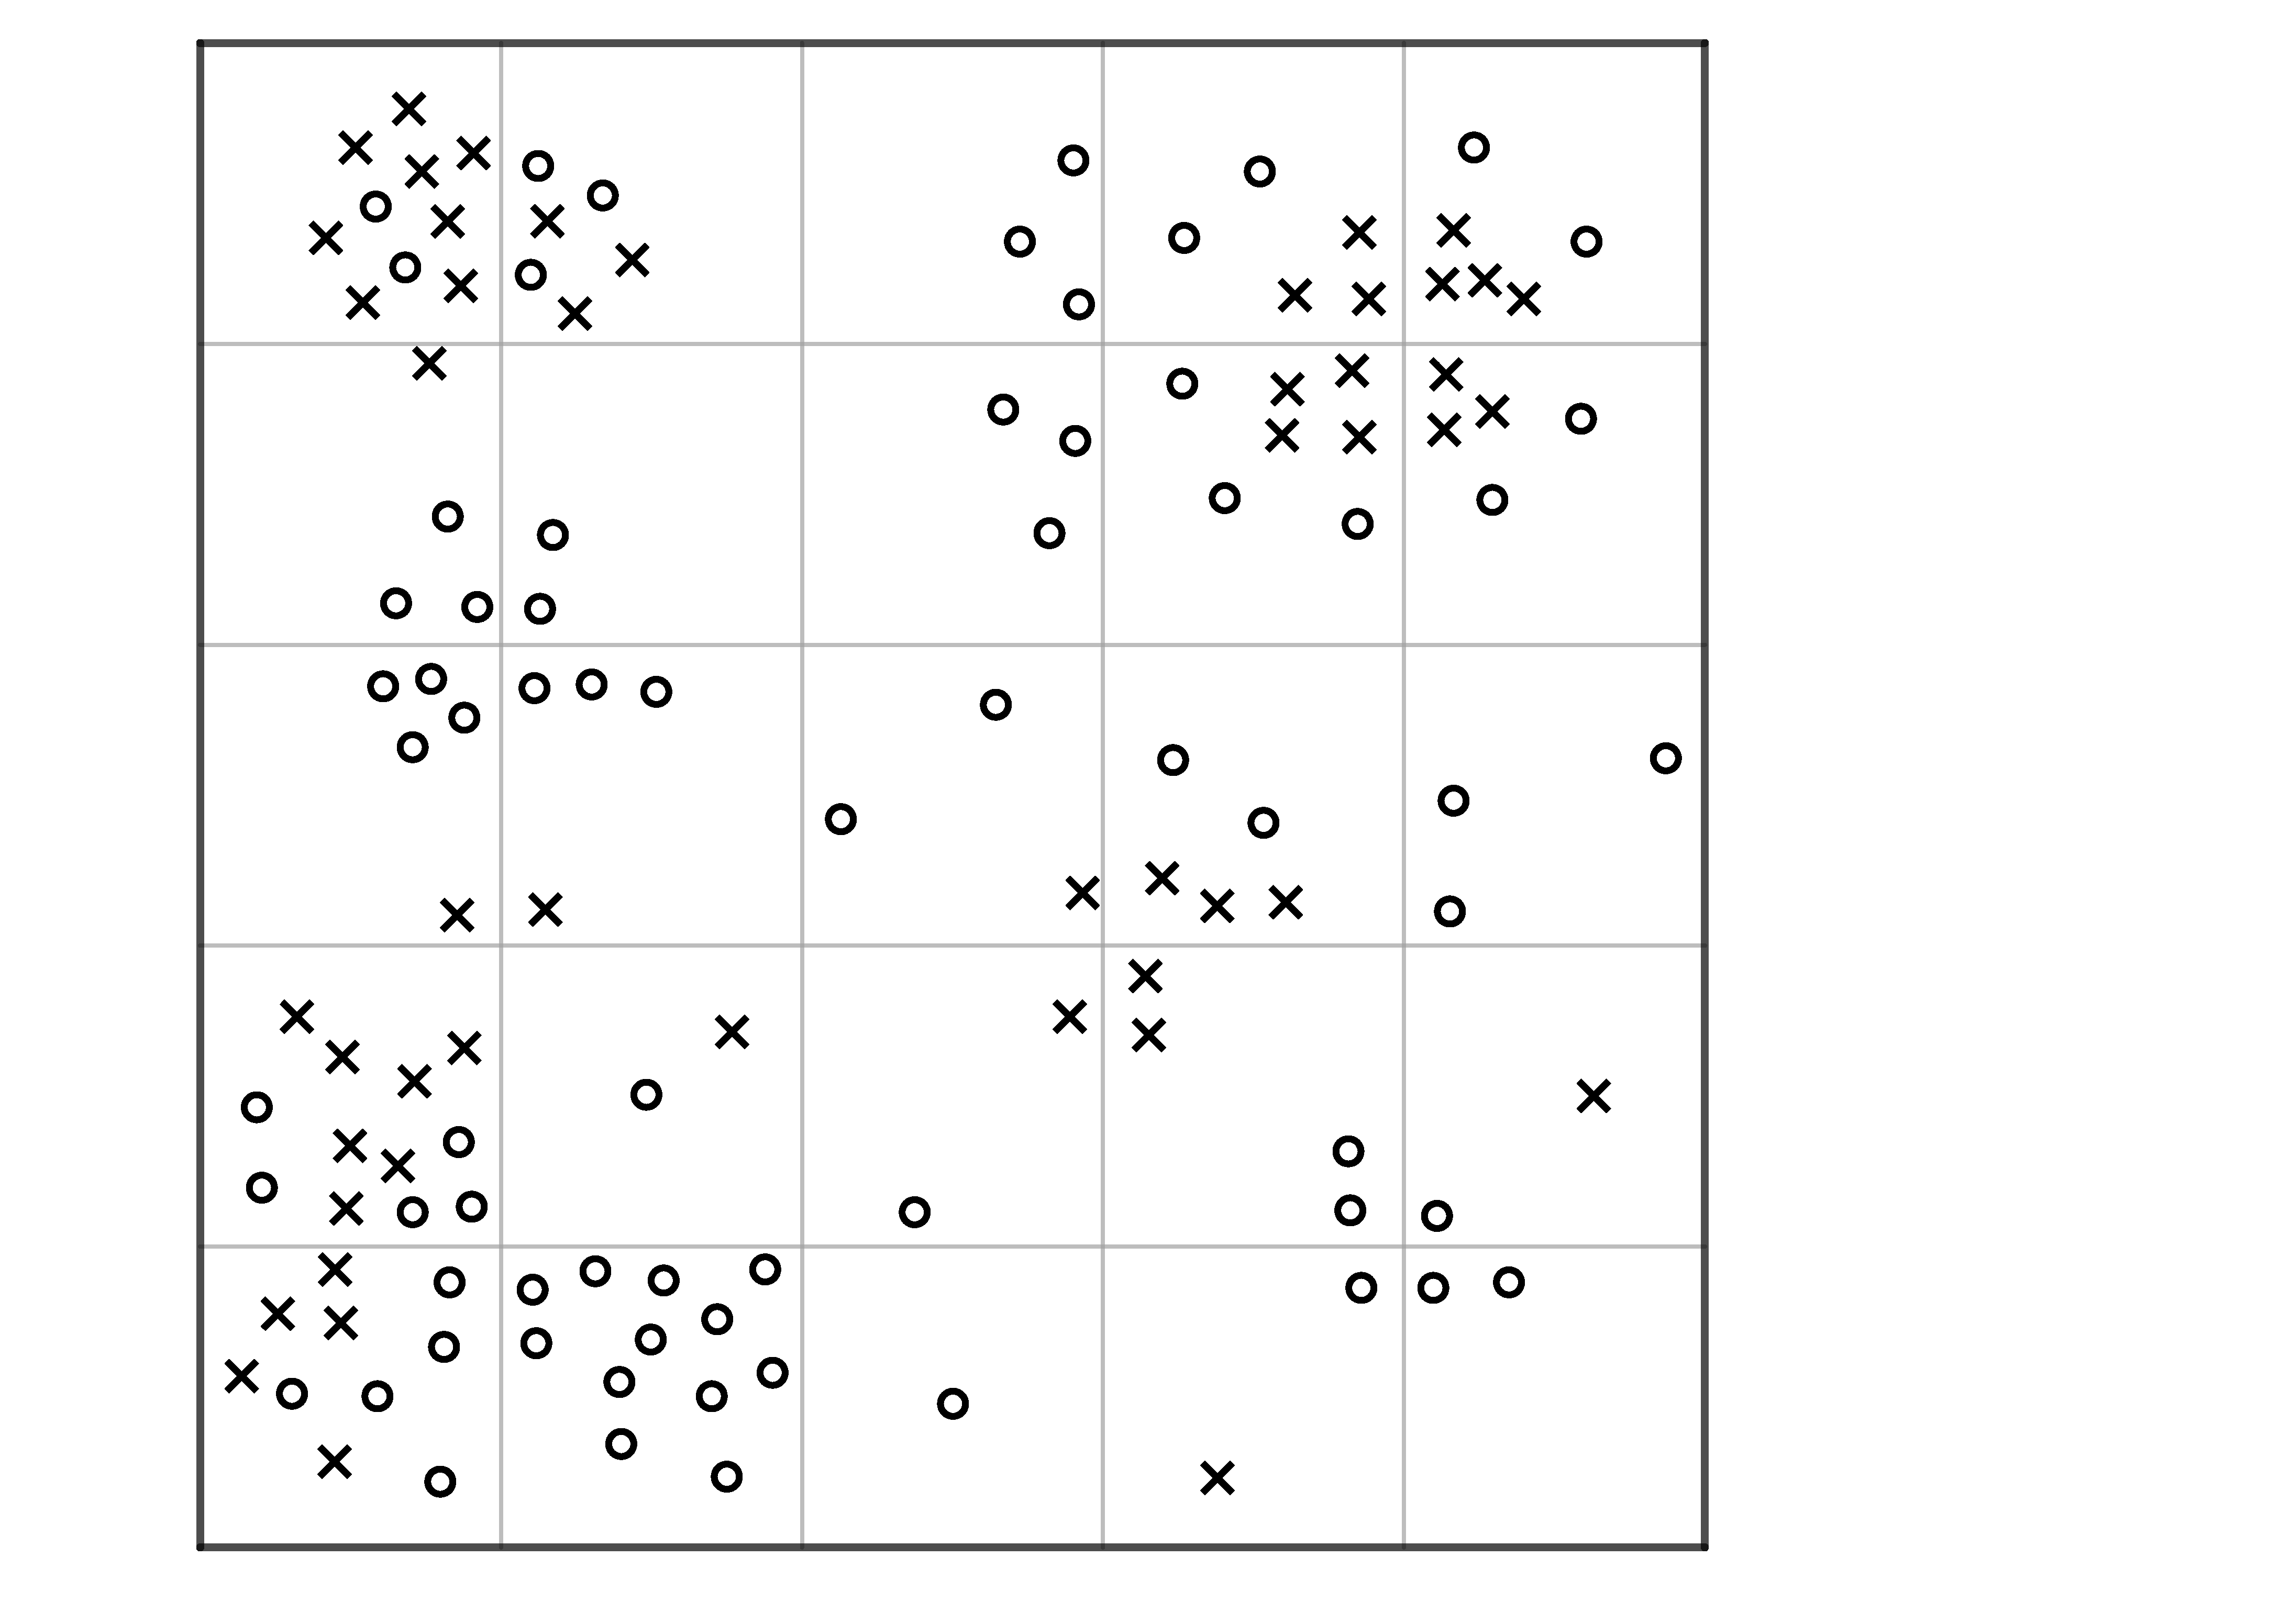
\includegraphics[width=2in]{Gerry5x5-120-3.pdf}\\
 Total Vote Count &  Total Vote Count &  Total Vote Count\\
 X -  45& X - 40 & X  - 50\\
 O - 75 & O - 80 & O - 70
 \end{tabular}


Province F\\
Population = 150
\begin{tabular}{c c c }

Year 1 & Year 2 & Year 3 \\
 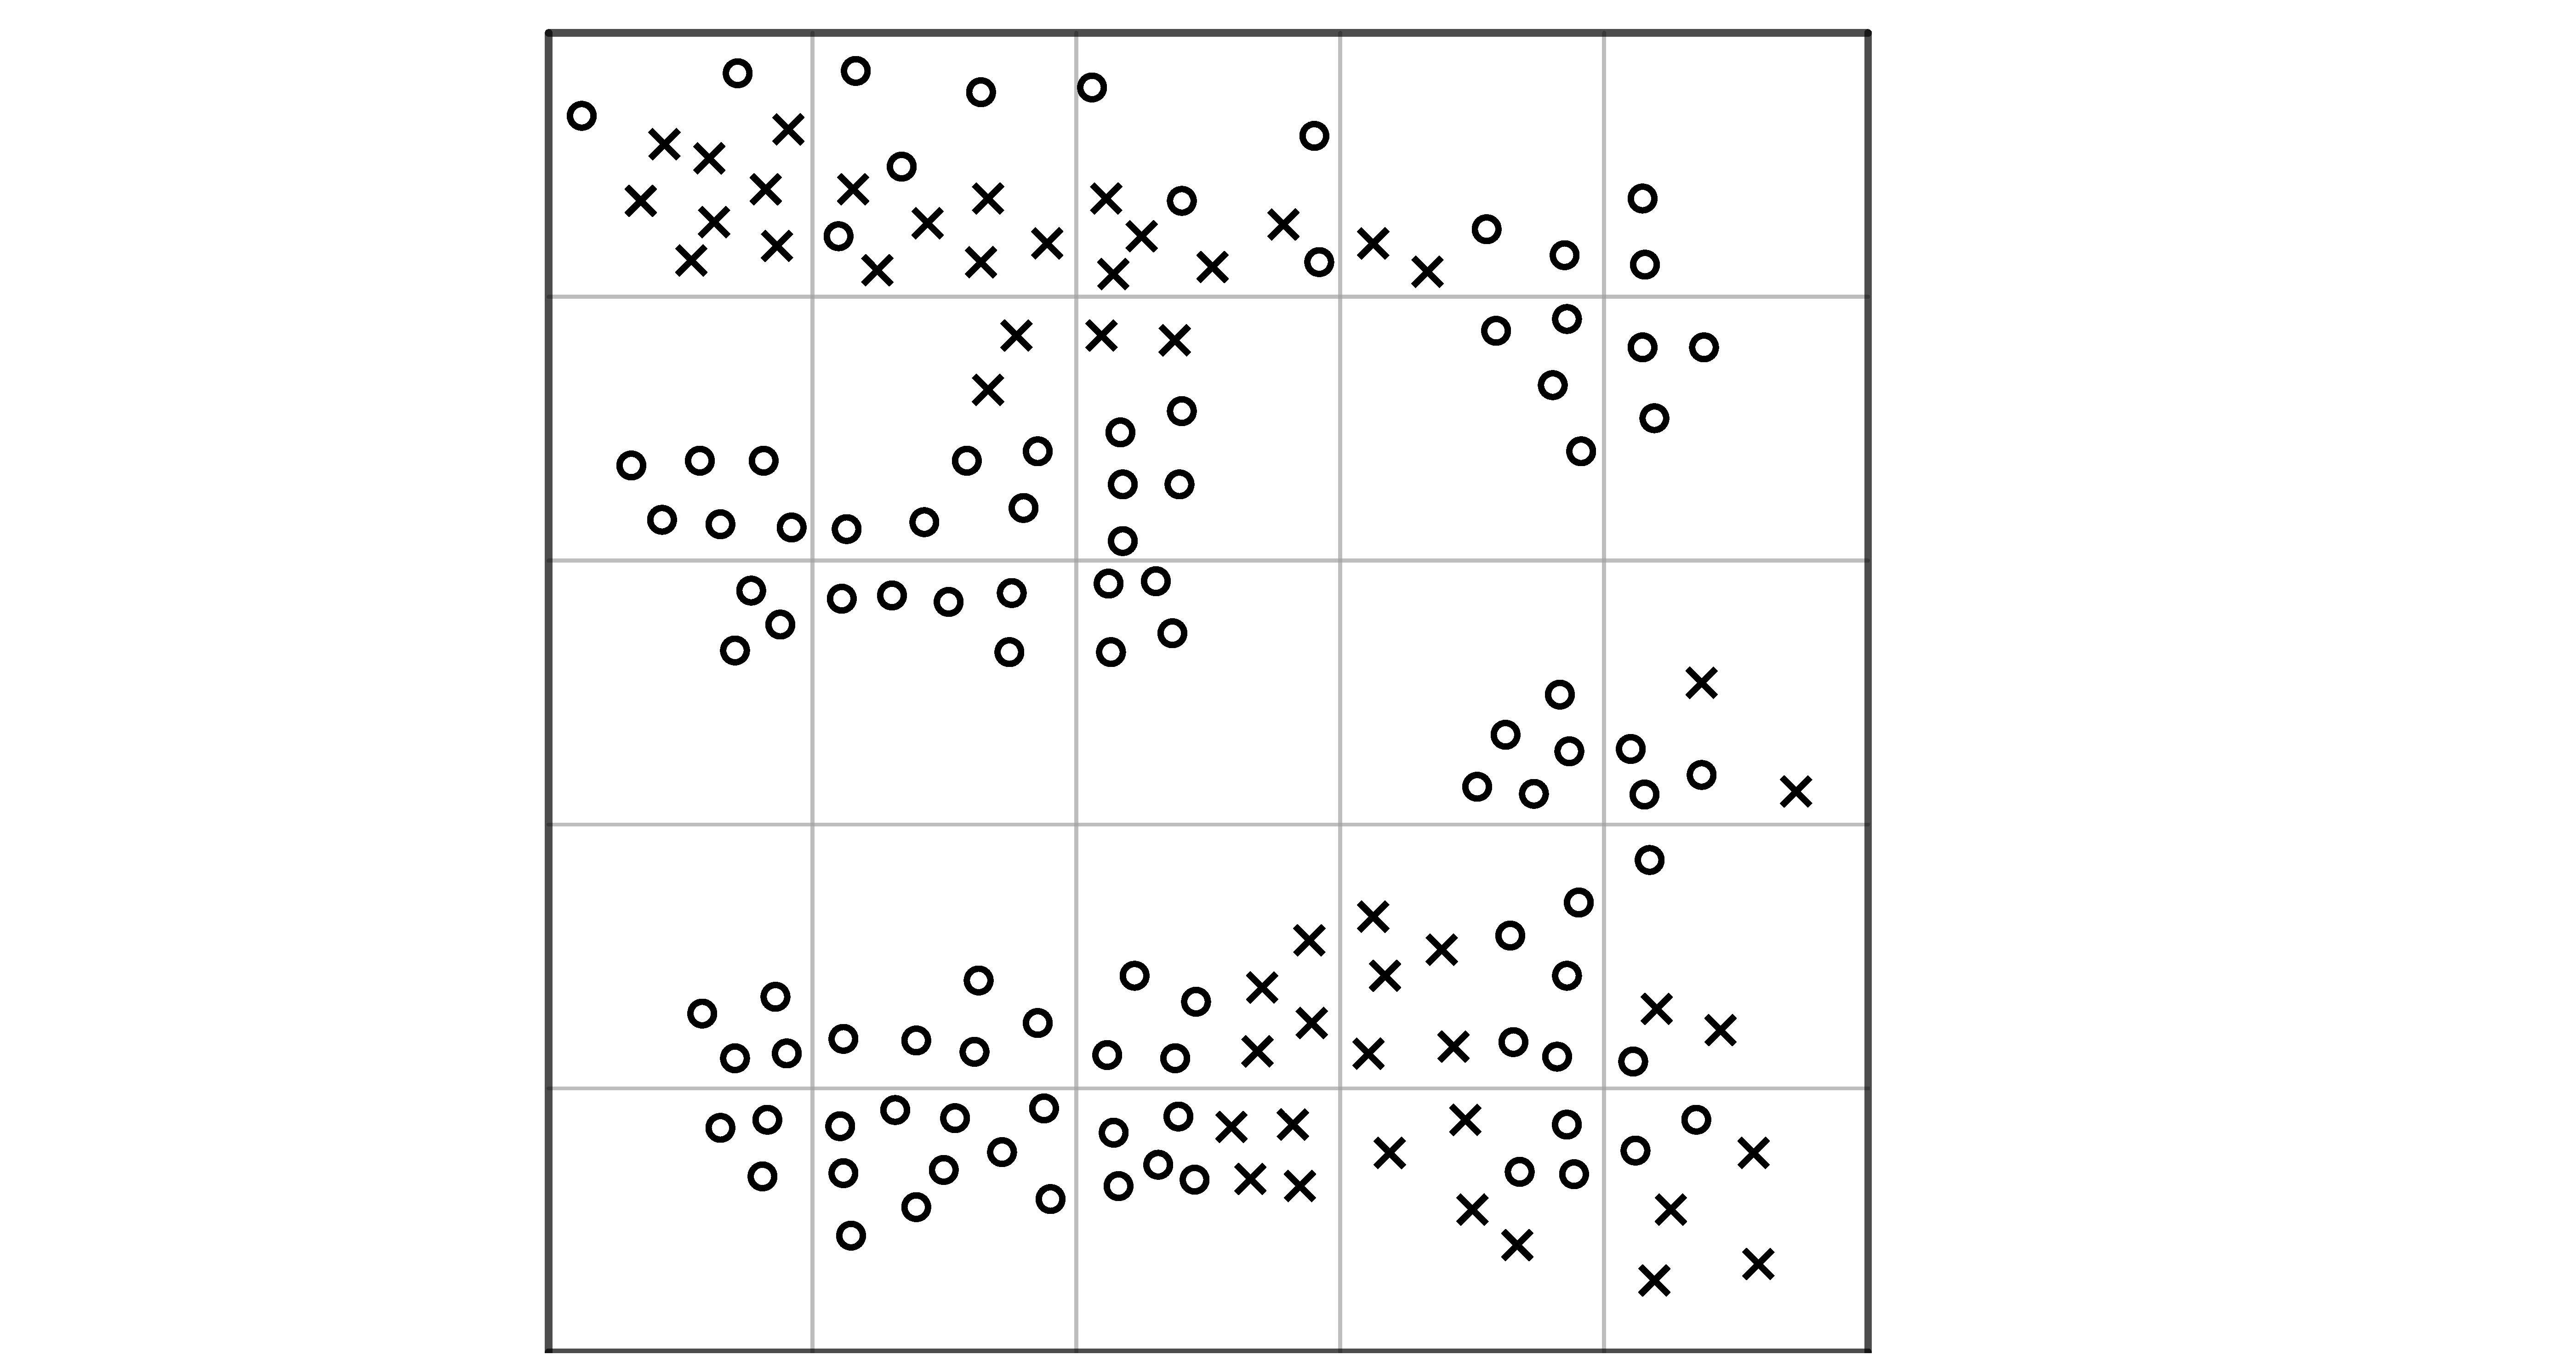
\includegraphics[width=2in]{Gerry5x5-150-1.pdf} &  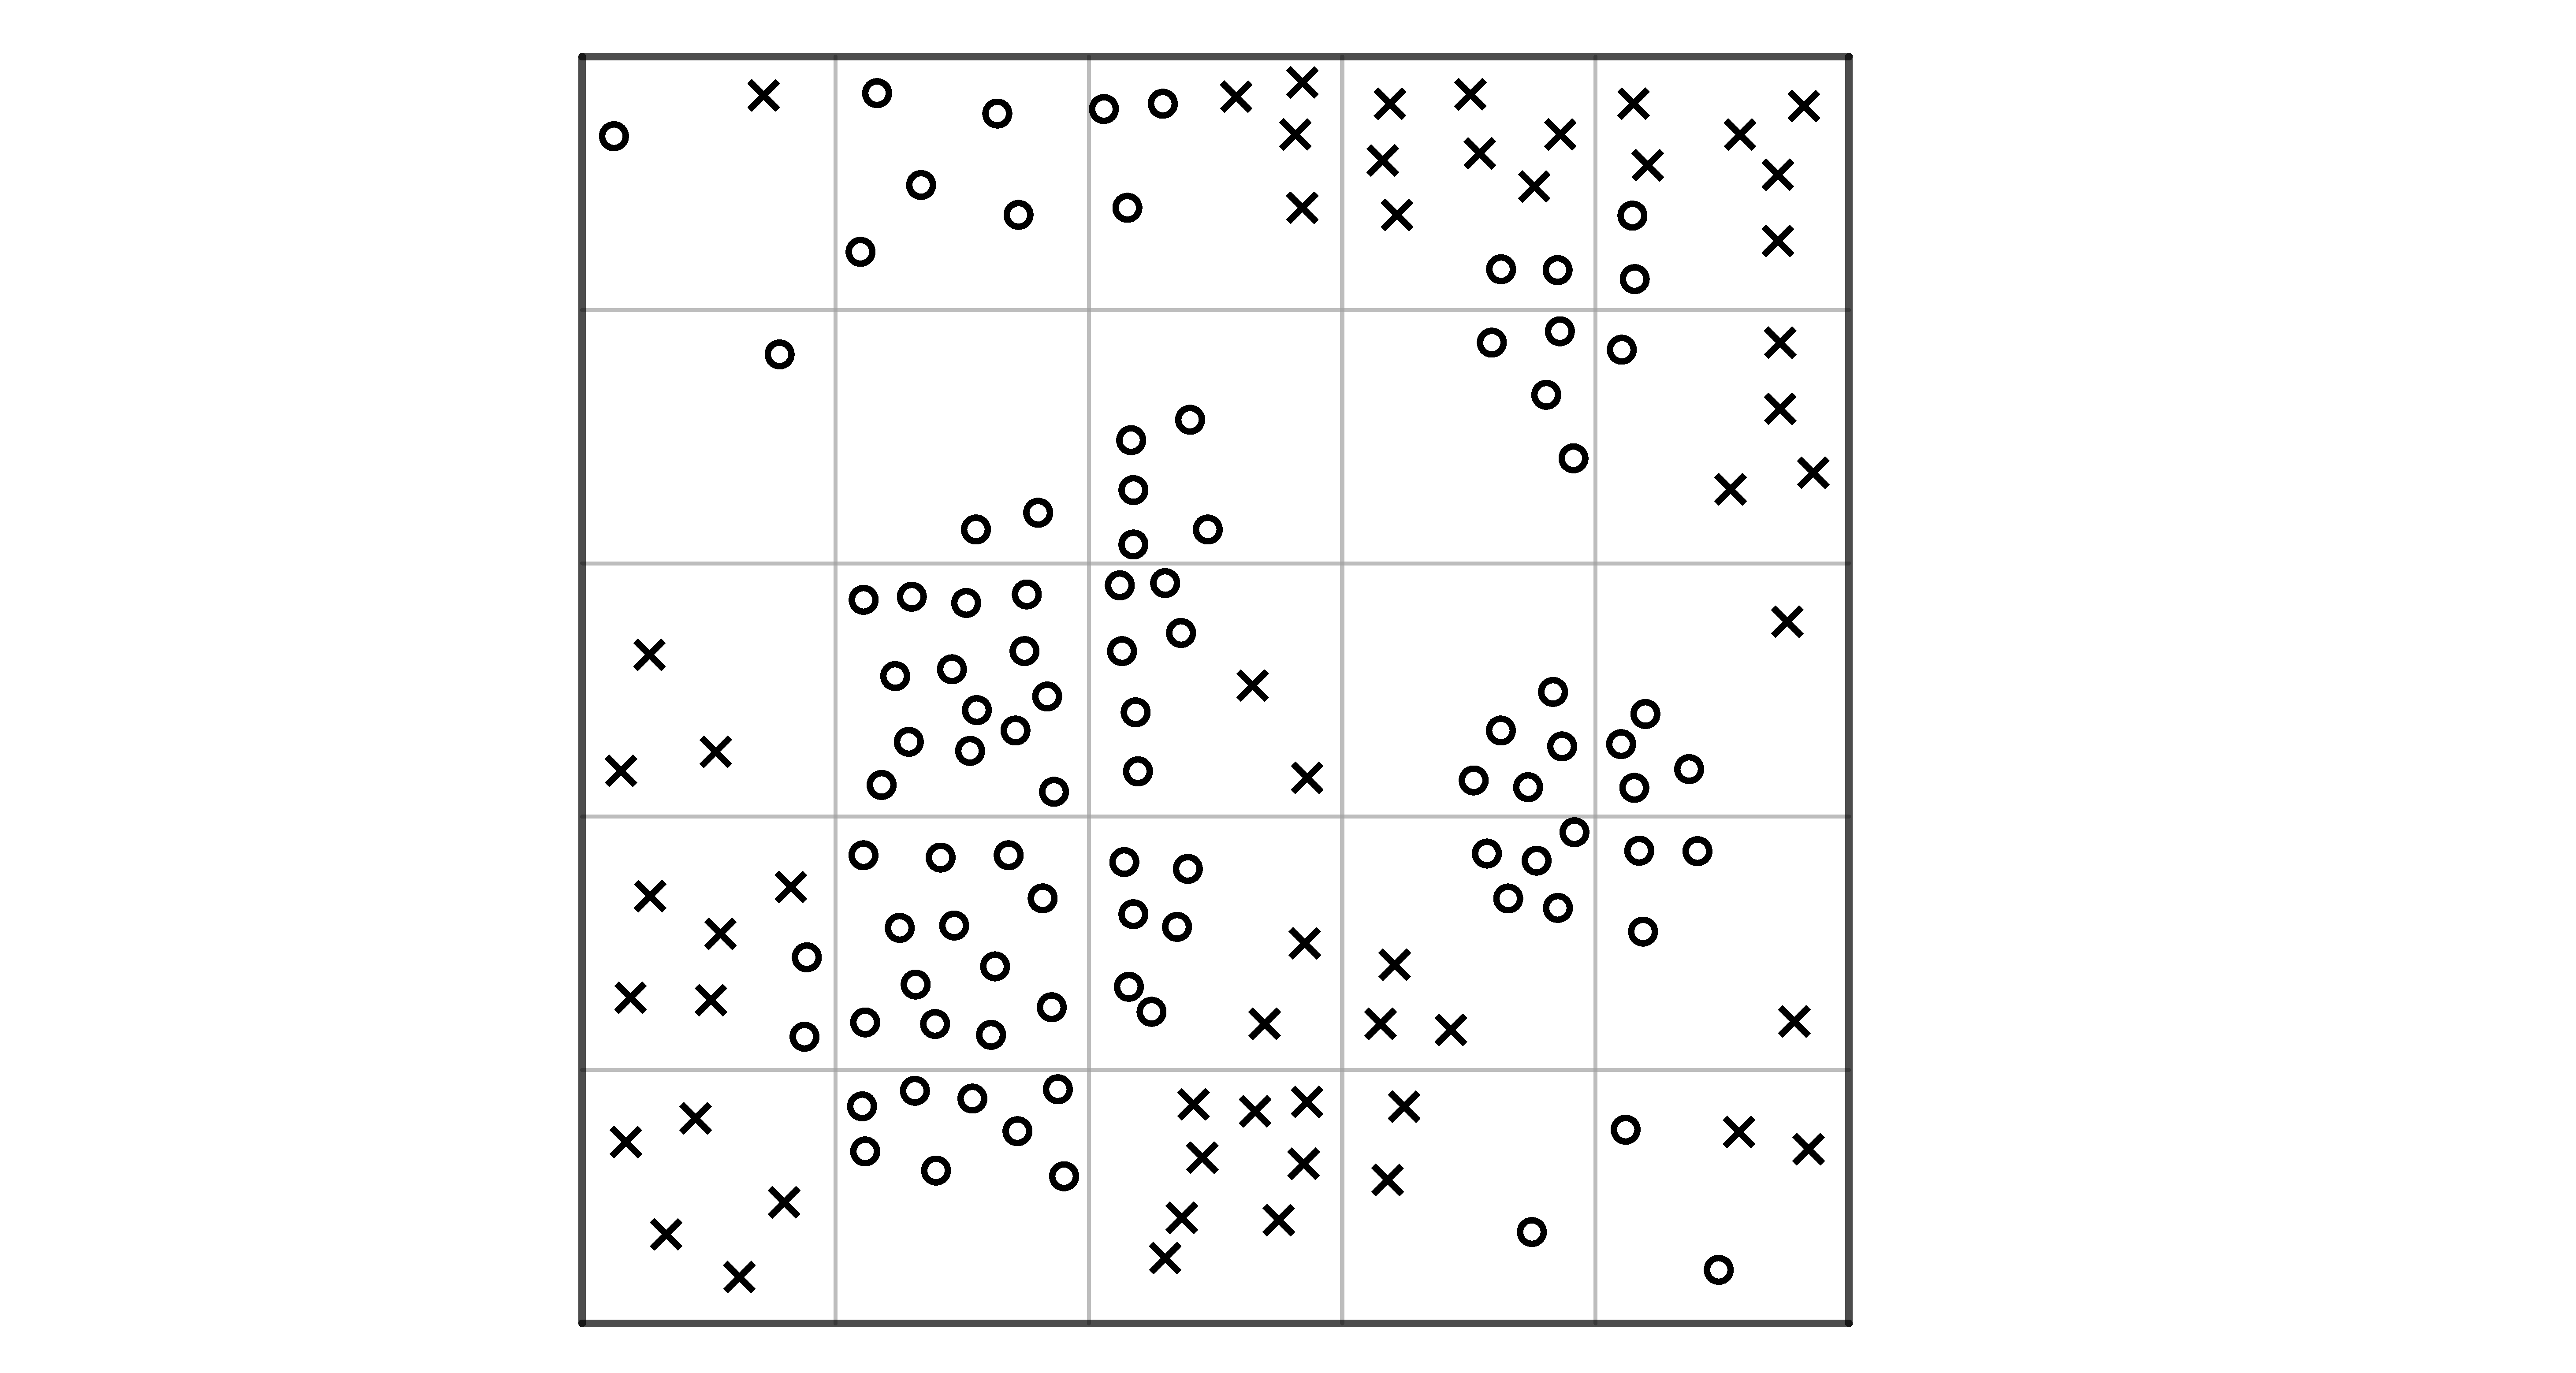
\includegraphics[width=2in]{Gerry5x5-150-2.pdf} &  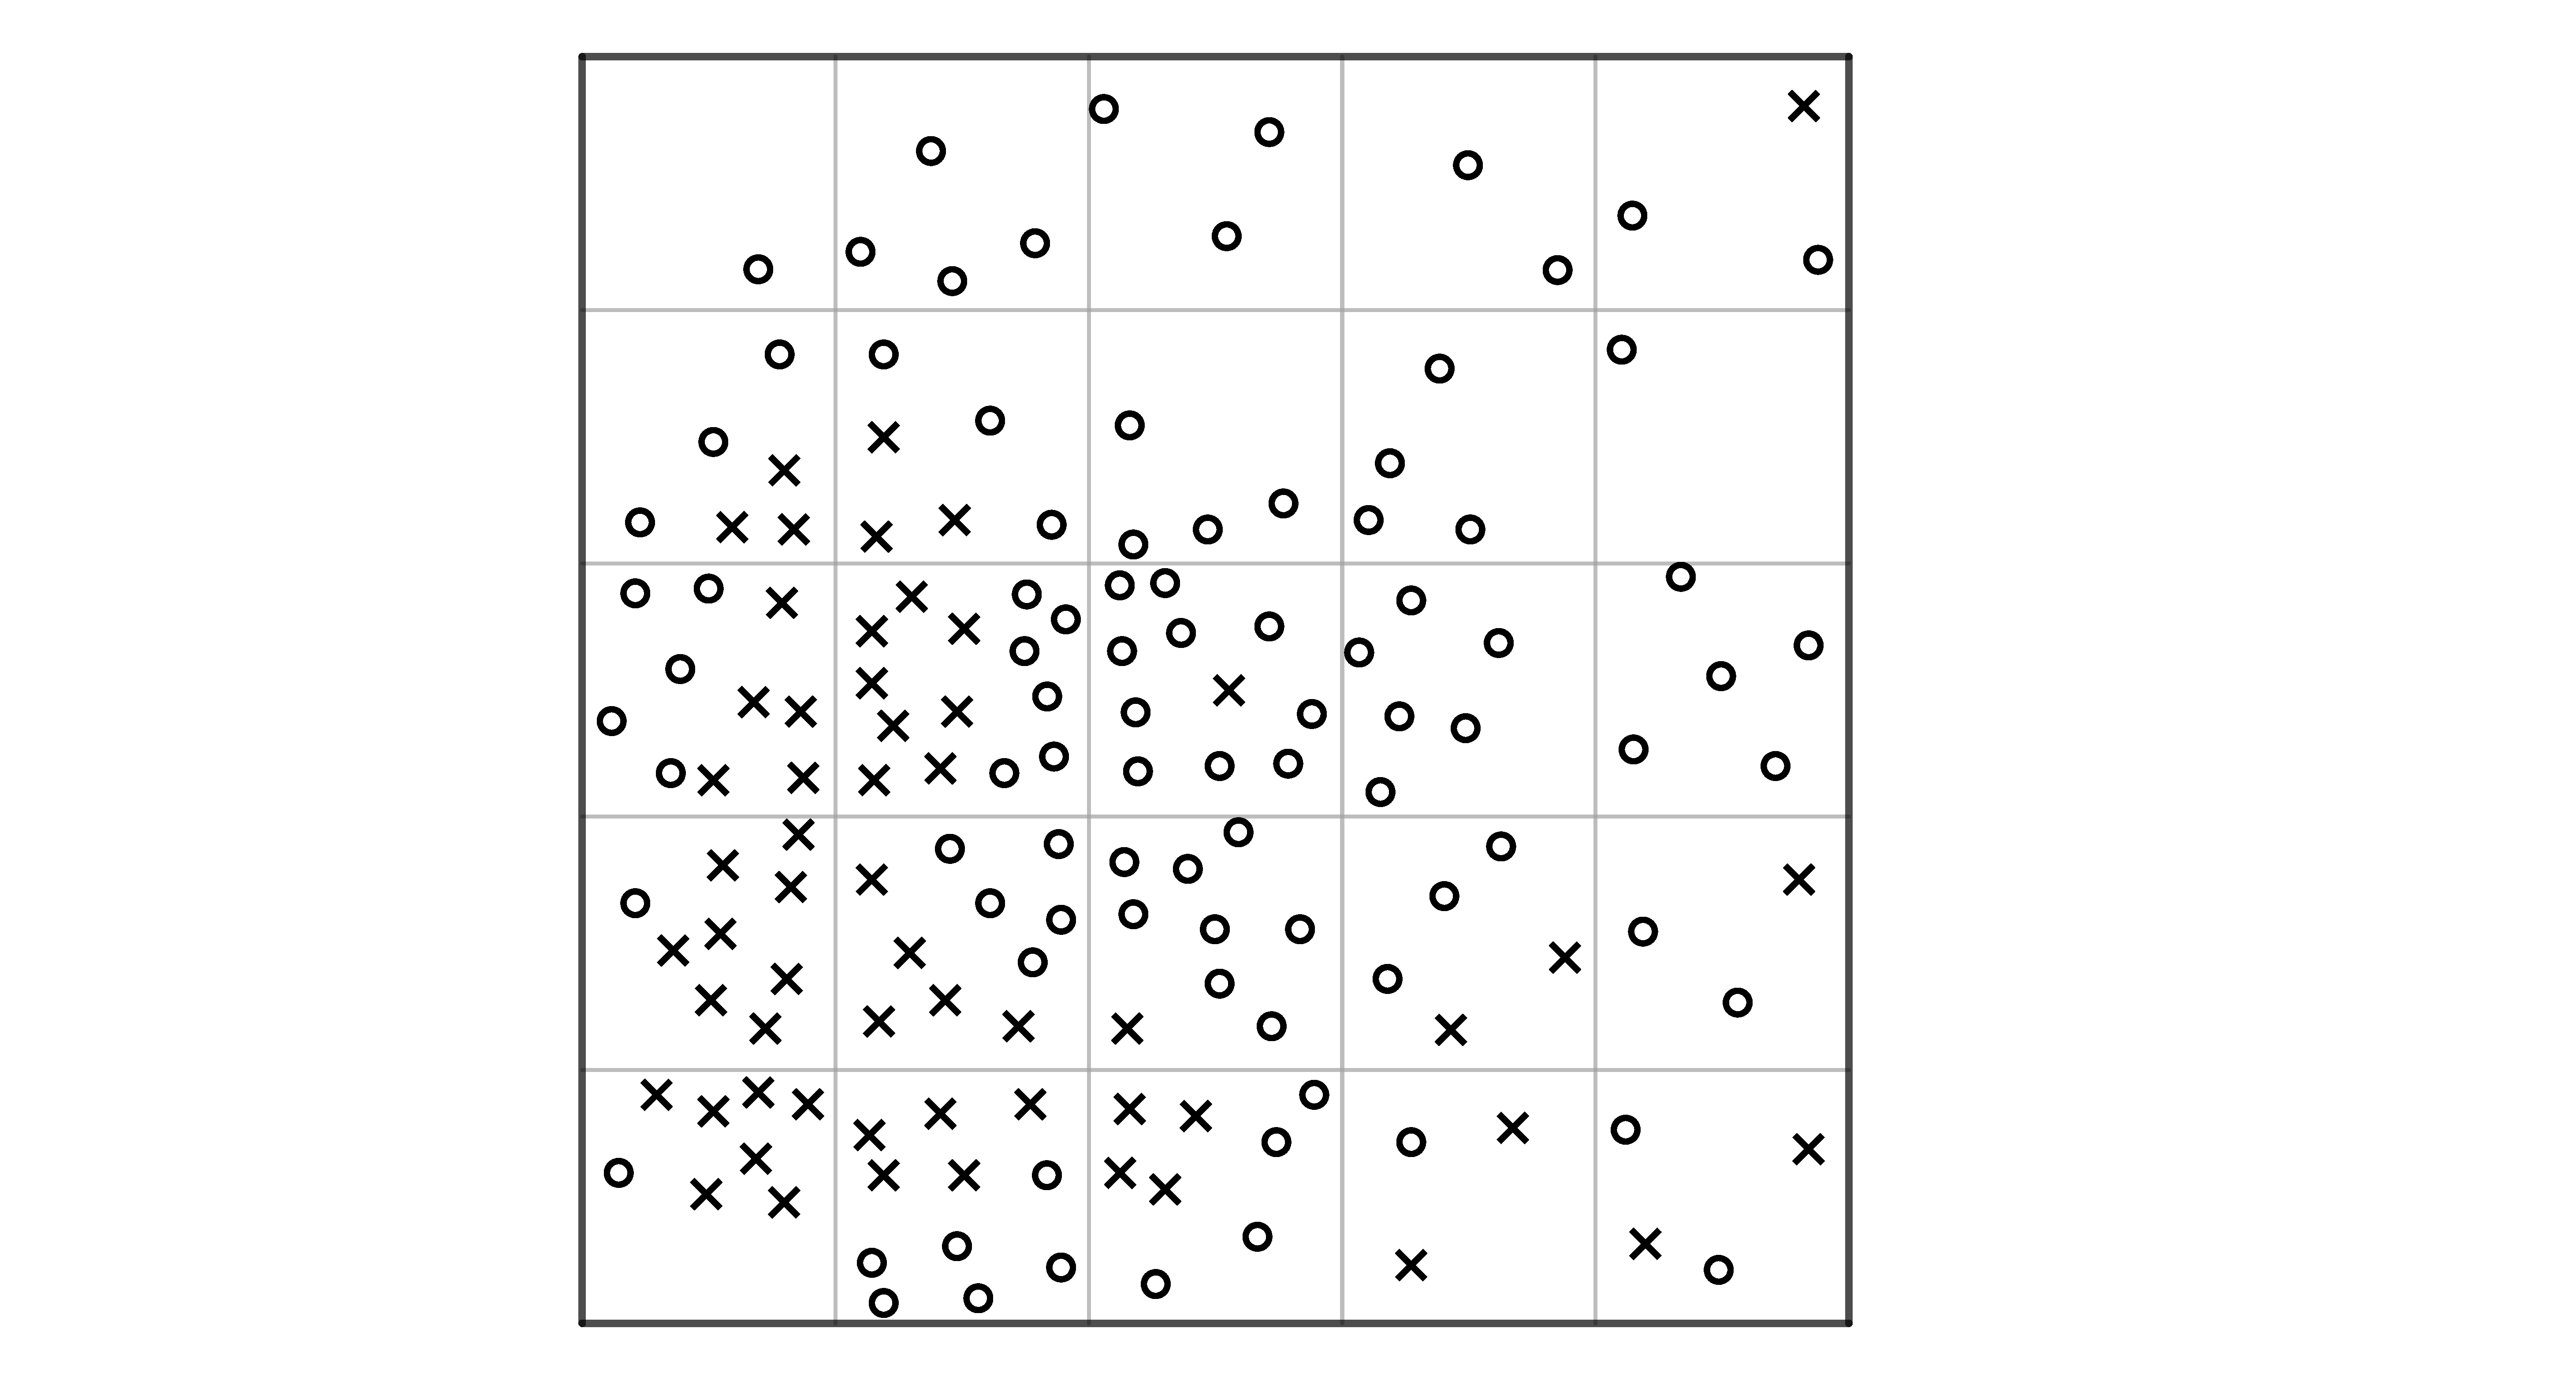
\includegraphics[width=2in]{Gerry5x5-150-3.pdf}\\
 Total Vote Count &  Total Vote Count &  Total Vote Count\\
 X -  50& X - 56 & X  - 58\\
 O - 100 & O - 96 & O - 92
 \end{tabular}
\end{flushleft}
\end{document}
